%%
%% elsarticle format. Compiler: pdfLaTex
%% elsarticle.cls is modified to avoid errors.

\documentclass[preprint,11pt,authoryear]{elsarticle}

%% Use the option review to obtain double line spacing
%\documentclass[authoryear,preprint,review,12pt]{elsarticle}

%% Use the options 1p,twocolumn; 3p; 3p,twocolumn; 5p; or 5p,twocolumn
%% for a journal layout:
%% \documentclass[final,1p,times,authoryear]{elsarticle}
%% \documentclass[final,1p,times,twocolumn,authoryear]{elsarticle}
%% \documentclass[final,3p,times,authoryear]{elsarticle}
%% \documentclass[final,3p,times,twocolumn,authoryear]{elsarticle}
%% \documentclass[final,5p,times,authoryear]{elsarticle}
%% \documentclass[final,5p,times,twocolumn,authoryear]{elsarticle}

% Graphics and figures
\usepackage{graphicx}
\usepackage{caption}
\usepackage{subcaption}
\usepackage{tikz}
\usetikzlibrary{arrows.meta,positioning,decorations.pathreplacing}


% Tables
\usepackage{booktabs}
\usepackage{longtable}
\usepackage{multirow}
\usepackage{threeparttable}
\usepackage{makecell}

% Mathematics
\usepackage{amsmath, amsfonts, amssymb}

% Link
\usepackage{url} 
\usepackage{hyperref}
\hypersetup{colorlinks = true,
linkcolor = blue,
anchorcolor =red,
citecolor = blue,
filecolor = red,
urlcolor = red,
pdfauthor=author}

\usepackage{mathpazo} %Use Palotino fonts

\usepackage{geometry}
\geometry{
 a4paper,
 total={170mm,257mm},
 %left=30mm,
 %top=25mm,
 bottom=20mm,
 }

\journal{European Economic Review}

\begin{document}

\begin{frontmatter}

\title{Anchored Abroad: Sunk Costs, Asset Specificity, and Japanese Affiliate Exit from Brexit Britain\tnoteref{t1}}
\tnotetext[t1]{First version: November 1, 2024. This version: \today.}

\author[inst1]{Michael Ryan\corref{cor1}}
\ead{michael.ryan@wmich.edu}

\author[inst2]{Ayumu Tanaka\corref{cor2}}
\ead{ayumu@aoyamagakuin.jp}

\affiliation[inst1]{organization={Department of Economics, Western Michigan University},
            addressline={1903 W. Michigan Ave}, 
            city={Kalamazoo},
            postcode={49008}, 
            state={MI},
            country={USA}}

\affiliation[inst2]{organization={College of Economics, Aoyama Gakuin University},
            addressline={4-4-25 Shibuya}, 
            city={Shibuya-ku},
            postcode={150-8366}, 
            state={Tokyo},
            country={Japan}}

\cortext[cor1]{Corresponding author. ORCID: 0000-0001-9381-3112.}
\cortext[cor2]{ORCID: 0000-0001-9858-9236.}

\begin{abstract}
This paper examines Brexit's impact on foreign direct investment (FDI) in the United Kingdom (UK), with a specific focus on affiliate exit and divestment behavior.
It is among the first to provide micro-level evidence on FDI exit behavior post-Brexit, offering new insights into the role of sunk costs and hysteresis in multinational location strategies.
Our theoretical framework demonstrates that substantial sunk costs create hysteresis effects that asymmetrically impact entry and exit decisions. 
To test this, we employ state-of-the-art difference-in-differences and synthetic difference-in-differences methodologies to compare Japanese affiliates in the UK with those in other European states, using comprehensive Japanese FDI data spanning 2010--2020.
While Brexit significantly reduced new market entry, existing affiliates exhibited remarkable persistence despite reduced UK market potential. 
Heterogeneity analysis reveals stronger hysteresis effects in high asset-specificity industries. Results remain robust across multiple econometric specifications, challenging prevailing narratives about Brexit's detrimental FDI effects and highlighting investment irreversibility's critical role in multinational location strategies even after a large policy shock.\\
\end{abstract}


%%Research highlights
\begin{highlights}
\item Brexit had little effect on Japanese UK exits, defying fears of a mass foreign exodus.
\item Robust DiD and SDiD results show how Japanese firms responded to Brexit over time.
\item Brexit reduced new Japanese UK entries, but did not cause more existing firm exits.
\item Sunk costs explain why Japanese firms stayed in post-Brexit UK despite lower appeal.
\item Exit rates rose in low-specificity sectors but stayed stable where assets were sunk.
\end{highlights}



\begin{keyword}
Brexit \sep FDI \sep exit \sep divestment \sep difference-in-differences \sep hysteresis

\noindent
\textit{JEL-Classification:} F21, F23, F15, D22
\end{keyword}

\end{frontmatter}

%%%%%%%%%%%%%%%%%%%%%%%%%%%%%%%%%%%%%%%%%%%%%%%%%%%%%%%%%%%%%
%%%%
\section{Introduction}
\label{sec:introduction}
Brexit --- the process by which the United Kingdom (UK) exited the European Union (EU) in 2020 --- is one of the major economic and political events of the last decade.\footnote{The term ``Brexit" is generally attributed to Peter Wilding, BSkyB director of European policy, dating to May 2012. A growing Euroscepticism existed in the UK Conservative Party and UK Independence Party in the early 2010s. In January 2013, British Prime Minister David Cameron promised that the UK government would renegotiate its EU agreement if his party won the majority in the 2015 general election. Parliament did not consider the European Union (Referendum) Bill 2013 after January 2014, but it was reintroduced in the European Union Referendum Act 2015.} Brexit dominated the news for years for a variety of reasons, not the least being that Brexit represented the first significant situation of a country unilaterally leaving a customs union. 
Importantly for this paper, among the numerous Brexit-related issues were the questions regarding how foreign investors would treat the UK's withdrawal from the EU. The potential loss of inward foreign direct investment (FDI) concerned not only British economists and policymakers but also current and prospective foreign investors. 

Notably, the Japanese government raised key concerns in a \textbf{post-referendum} letter sent to both the UK and EU governments. This letter outlined the fears many foreign firms and governments had regarding the UK's exit, especially concerning the predictability and \textbf{transparency of the institutional changes expected after the referendum}.\footnote{See ``Japan’s Message to the United Kingdom and the European Union." by the Government of Japan, \url{https://www.mofa.go.jp/files/000185466.pdf}. Last accessed: 9 December 2024.} Japan, traditionally one of the largest sources of global outward FDI, was (and continues to be) a major source of investment into the UK and EU. Concern over the future UK and EU investment landscape was significant and the government communique noted that ``... many other foreign firms that have invested in the UK, each of which is quite capable of upping sticks in the next phase of their investment cycle."\footnote{``Britain cannot easily dismiss Japanese Brexit warning letter," \textit{The Guardian}, \url{https://www.theguardian.com/politics/2016/sep/04/britain-japanese-brexit-letter-eu}.  Last accessed: 9 December 2024. See also ``Japan's Brexit demands range from possible to fanciful,"  \textit{The Guardian}, \url{https://www.theguardian.com/world/2016/sep/04/japan-brexit-demands-range-from-possible-to-fanciful}. Last accessed: 9 December 2024.} In this context, ``upping sticks" indicates the parent firm pulling its affiliate out of the UK, likely for other locations within the EU.  
Similarly, news articles sounded the alarm over firms exiting the UK. 
Headlines such as this in the CNN --- ``Japan Inc poured billions into Britain. Now it's having regrets.''\footnote{\textit{CNN}, \url{https://www.cnn.com/2019/02/19/business/japan-companies-uk-economy/index.html}. Last accessed: 9 December 2024.} were prominent. Similarly, a Politico.eu article noted ``Brexit triggers exodus of Japanese firms from UK to EU.''\footnote{\textit{POLITICO}, \url{https://www.politico.eu/article/brexit-trade-japan-exodus-firms-uk-eu/}. Last accessed: 9 December 2024.}

However, the credibility of the ``upping sticks" threat could be questioned, because behind all the bluster of government reports and news headlines, much more subtle changes were actually occurring. While Nissan did cease some production at its Sunderland plant, this was in part because of the ``withdrawal of its luxury marque from Western Europe in the face of competition from Germany's carmakers."\footnote{\cite{maidment2019brexit}.} Financial firms such as Mitsubishi UFJ, Daiwa, Mizuho Financial Group, and Sumitomo Mitsui Financial expanded their European operations, although they often kept UK-based affiliates; in some cases, they even expanded UK operations. Moreover, few new Japanese manufacturing facilities have been established in the UK, although ``non-automotive manufacturing employment and investment has stayed steady."\footnote{Pernille Rudlin (2023). ``Japanese Companies in The UK 7 Years On – The New Third Phase," Rudlin Consulting Ltd, \url{https://rudlinconsulting.com/japanese-companies-in-the-uk-7-years-on-the-new-third-phase/}.}

Pushing past the headlines, an understanding of how foreign affiliates actually reacted to \textbf{the uncertainty following the Brexit referendum} can lead to improved policy when the next such customs union exit occurs. While gloomy projections existed and research indicates that the Brexit vote caused a UK output loss of 1.7\% to 2.5\% by year-end 2018, --- a period following the 2016 referendum but prior to the formal exit (e.g., \citealt{born2019}) --- did multinational enterprises (MNEs) follow through on the threats of ``upping sticks" and leave the UK at a greater rate than before the announcement? Or, in contrast to closing affiliates, did Japanese MNE parents partially divest their equity holdings in previously established affiliates to minimize Brexit-related risks? 

Our model highlights \textbf{how policy uncertainty interacts with sunk costs} to influence FDI decisions, particularly in determining entry and exit behavior. These factors create a wider hysteresis band that asymmetrically affects new investments and existing affiliates. Specifically, while \textbf{Brexit uncertainty} may have deterred new investment into the UK, it did not necessarily trigger widespread exits among established affiliates. Even if the UK’s market attractiveness declined \textbf{post-referendum}, hysteresis effects likely constrained the ability or willingness of firms to withdraw. This is because shutting down an existing affiliate involves abandoning sunk assets, making exit costly. In contrast, potential investors can more easily abandon new investment plans before committing to those sunk costs.


Now, more than nine years since the Brexit referendum of 2016, and five years since the UK officially left the EU in 2020, this paper examines how Japanese \textbf{MNE parents have responded to the uncertainty triggered by the Brexit referendum}. In contrast to the significant literature that has examined the macroeconomic impacts of Brexit, particularly \textbf{post-referendum}, this paper uses affiliate-level data to examine how Japanese UK-based affiliates were affected by \textbf{the Brexit referendum}. We explore whether Japanese affiliates left the UK as the government and some media predicted, or whether they remained in the UK, despite the diminished attractiveness of the UK as a host country for foreign investment.
Importantly, using a comprehensive micro dataset of Japanese affiliates for which we can identify annual changes in affiliate location and ownership structure, we compare the rate at which Japanese affiliates exited the UK relative to other EU member countries. Beyond examining exits, we analyze partial divestments from UK-based and other affiliates to identify additional, more nuanced Brexit-related behavioral differences.


We utilize Toyo Keizai Inc.’s Overseas Japanese Companies Data for our study, examining Japanese affiliates in the UK and other EU countries from 2010--2020. This dataset allows us to examine exit and divestment behavior at the affiliate level. Employing a variety of difference-in-differences (DiD) and synthetic DiD approaches, we investigate, for existing affiliates: (i) if full affiliate exit (affiliate closure) rates differed \textbf{post-referendum versus pre-referendum} within the UK, (ii), if divestiture (partial exit from an existing affiliate) increased \textbf{post-referendum} within the UK, and (iii) if these changes differed from Japanese MNE investment behavior within the remaining EU countries? In doing so, we identify the degree to which Japanese behavior within the UK differs from the rest of Europe, and how ownership changes of existing UK-based affiliates differ from that of affiliates in other EU countries. 
This allows us to identify how Japanese affiliates behaved differently in the UK as compared to the other EU countries.


To identify the causal impacts of \textbf{the Brexit referendum}, we employ a variety of state-of-the-art DiD methods. 
Relying on the standard identifying assumptions, we estimate the average treatment effect on the treated (ATT) via the two-way fixed effects (TWFE) model.
In addition, we use the extended TWFE model of \cite{wooldridge2021two} as the robustness checks.
We further use the synthetic DiD method which is robust to the possible violation of the parallel trends assumption.


Our results suggest that significant hysteresis effects in FDI do exist, as \textbf{the Brexit referendum} appears to have had no effect on Japanese affiliate exit from the UK, except in industries with low asset specificity. In general, there is no significant difference in the rate of \textbf{post-referendum} exits from the UK compared to other host countries, even after controlling for relevant covariates. Similarly, we find no apparent effect of \textbf{the Brexit referendum} on the ownership structure of UK-based affiliates in terms of divestment. These findings are robust across various DiD and SDiD specifications. However, we do find that \textbf{the Brexit referendum} has dampened new multinational entries into the UK. This asymmetry between entry and exit is consistent with our FDI model incorporating sunk costs.

This study advances the literature on Brexit and FDI by addressing critical gaps in understanding micro-level responses to a large policy shock. Our contributions are twofold.
First, we provide novel micro-level evidence on \textbf{the Brexit referendum's} impact on foreign affiliates in the UK, an area underexplored in prior studies. As \citet{dhingra2022expecting} review, most Brexit-related research on exports and FDI has focused on aggregate-level outcomes, while firm-level dynamics have received relatively little attention. For instance, \citet{kren2024} estimate that Brexit reduced trade between the United Kingdom and the European Union by nearly 20\% in both directions. Similarly, \citet{steinberg2019brexit} employ a dynamic general equilibrium model to estimate that uncertainty about post-Brexit trade policies led to a consumption-equivalent welfare cost for UK households ranging from 0.4\% to 1.2\%. However, both studies overlook microeconomic impacts.
Although \citet{breinlich2020} and \cite{cieslik2022brexit} analyze the impacts of \textbf{the Brexit referendum} on FDI flows, they focused on the aggregated number of new investments and outward FDI from the UK, rather than micro-level exit and divestment behaviors. By examining these underexplored dimensions, our study reveals micro-level responses critical for policymakers navigating \textbf{post-referendum} investment strategies.

Second, we disentangle the decrease in inward FDI into the UK after Brexit by examining both entry and exit margins. While previous literature such as \citet{breinlich2020} and \cite{cieslik2022brexit} has focused on decreased entry, our analysis reveals that the exit channel plays a limited role --- Japanese affiliates do not exit the UK market significantly more after Brexit than before. To explain this asymmetric pattern, we underscore the role of sunk costs in FDI decisions, extending insights from export-focused studies \citep{roberts1997decision, das2007market, handley2015trade, graziano2021brexit}. While sunk costs are well-documented in exporting, their impact on FDI decisions remains understudied. We address this gap by developing a simple theoretical model incorporating sunk costs and hysteresis effects, which predicts asymmetric Brexit impacts on new entrants and existing affiliates. Specifically, high sunk costs deter new FDI while encouraging existing affiliates to persist despite adverse conditions, offering a framework to assess long-term investment dynamics. Our empirical part largely confirms the model predictions.

The remainder of the paper is organized as follows.
Section~\ref{sec:Model} presents a simple model of FDI with sunk costs, which illustrates the asymmetric effects of \textbf{the Brexit referendum} on new entry and exit. Section~\ref{sec:data} describes the data and provides preliminary analysis, while Section~\ref{sec:method} outlines the empirical methodology. Section~\ref{sec:results} reports the baseline results, and Section~\ref{sec:robustness} offers robustness checks. Section~\ref{sec:mechanism} explores the underlying mechanisms driving the baseline findings. Section~\ref{sec:conclusion} concludes.
The Appendix includes descriptive statistics for the variables used in the main regressions, a list of host countries, maps showing the locations of Japanese affiliates in the UK and other EU countries, and the industry classification based on asset specificity. 
The Online Appendix provides additional descriptive statistics and the results from Cox proportional hazard models.



\section{A simple model of FDI with sunk costs}\label{sec:Model} 

\subsection{Background}

The UK finally left the EU on January 31, 2020, after it unexpectedly voted to leave the EU in a referendum held on June 23, 2016.
Even before the official exit in 2020, Brexit had already reduced the UK's attractiveness as a host country for FDI due to the uncertainty surrounding the future UK-EU trade relationship. 
\cite{dhingra2022expecting} conclude that the "Leave" vote had a sizable negative effect on the UK economy even before the country formally exited the EU. Summarizing the results of the previous studies, they argue that the Brexit referendum reduced the size of the UK economy by around 2--3\% by the end of 2019.
This decline is attributed to uncertainty and the expectation of higher future barriers to trade and migration, which led to lower capital investment, weaker demand, and slower GDP growth.

How the reduction in the UK's attractiveness as a host country for FDI affects foreign firms' investment decisions is an important question. 
We propose a simple model of FDI with sunk costs to explain the impacts of Brexit on affiliate exits.
Investment irreversibility is crucial to understand affiliate exit behavior.\footnote{While \cite{garetto2019} develop a comprehensive dynamic model to analyze the expansion patterns of multinational enterprises in time and space, our study focuses specifically on the exit margin following a large negative policy shock. Unlike their framework, which characterizes the global growth strategies of firms, we examine how the interplay between sunk costs and policy uncertainty creates hysteresis, leading to the observed persistence of existing affiliates despite deteriorating business conditions.}
According to \cite{kim2017asset}, disinvestment is more costly than new investment when investment is irreversible.
Several studies have investigated the role of sunk costs in exporting decisions \citep{roberts1997decision,das2007market,handley2015trade,graziano2021brexit}. However, in comparison to the extensive research on exporting behavior, studies explicitly focusing on the role of sunk costs in FDI decisions are less prevalent. This notable research gap highlights the need for further investigation into this important aspect to enhance our understanding of FDI determinants.

\subsection{FDI dynamics with sunk costs}

To explain the asymmetric impacts of Brexit, we present the dynamic discrete-choice model of FDI decisions by extending previous studies on exporting (e.g., \citealt{graziano2021brexit} and \citealt{roberts1997decision}). The model incorporates sunk costs, which create hysteresis in FDI participation.\footnote{\cite{graziano2021brexit} present closely related model to our model, as they also model exports with sunk costs to study the impacts of the Brexit referendum on UK-EU exports and net export entry. However, their focus is on export decisions, while we focus on FDI decisions. \cite{tamberi2024export} also develops a model of export-platform FDI under trade policy uncertainty and finds that Brexit uncertainty significantly discouraged new greenfield investment projects in the UK's manufacturing sector. However, while \cite{tamberi2024export} primarily focuses on the entry margin of new investment projects, our model explicitly incorporates exit costs and the irreversibility of investment to examine the exit margin.} 
The model is as follows. Suppose foreign parent firm $i$ is, in period $t$, choosing whether to undertake FDI by establishing an affiliate in host country $h$. The expected gross profit differential from FDI versus no FDI is:
$$
\pi_i(a_{ht}, \mathbf{z}_{it}),
$$
where $a_{ht}$ is the business conditions term which reflects both policy components and demand shifter. 
Therefore, $a_{ht}$ includes a host country's market potential and the trade policy factor (e.g., tariffs or non-tariff barriers).
We assume that the trade policy factor affects FDI profitability by limiting the export platform nature of FDI.
$\mathbf{z}_{it}$ captures firm-specific states such as FDI status. Brexit reduces $\pi_i(a_{ht}, \mathbf{z}_{it})$ by diminishing the UK's market potential, reflecting losses in EU market access and increased trade costs.\footnote{We do not impose a specific functional form on $\pi_i(a_{ht}, \mathbf{z}_{it})$, but it can be interpreted within the broader framework of FDI models, such as that proposed by \cite{head2021united}. More specifically, following \cite{graziano2021brexit}, we can consider the specific profit function as $\pi_{i}\left(a_{h t}, \mathbf{z}_{i t}\right)=D_{h t} \tau_{h t}^{-\sigma} c^{1-\sigma} \tilde{\sigma}$, where $D_{h t}$ is the demand shifter, $\tau_{h t}$ is the trade
policy factor, and the marginal cost $c$ is a component of the firm-specific state vector $\mathbf{z}_{i t}$. $\sigma$ is the elasticity of substitution, $\rho=(\sigma-1)/\sigma$, and $\tilde{\sigma}=(1-\rho)\rho^{\sigma-1}$.}



A parent firm incurs an initial entry cost of $F_i^{Entry}$ when establishing an affiliate for the first time. It represents, for example, costs for factory setup and obtaining necessary permits and licenses. It is a sunk cost, meaning it cannot be recovered if the affiliate exits the market. The parent firm also incurs an exit cost $F_i^{Exit}$ when it closes an affiliate in a host country. 

The FDI decision is represented by an indicator variable:
$$
FDI_{iht} = 
\begin{cases}
1 & \text{if the parent firm operates an affiliate in country } h  \text{ in period } t; \\
0 & \text{otherwise}.
\end{cases}
$$

For analytical tractability, we abstract from the possibility of re-entry after exit. With re-entry excluded, the parent firm's FDI history, $\mathbf{FDI}_{iht}^{(-)}$, depends solely on the previous period's status, $FDI_{ih,t-1}$. The period-$t$ profit is:
$$
R_{iht}(FDI_{ih, t-1}) = FDI_{iht} \left[ \pi_{iht} - F_i^{Entry} (1 - FDI_{ih,t-1}) \right] - F_i^{Exit} FDI_{ih,t-1} (1 - FDI_{iht}),
$$
where $\pi_{iht} \equiv \pi_i(a_{ht}, \mathbf{z}_{it})$. $F_i^{Entry} (1 - FDI_{ih,t-1})$ imposes the entry cost for new entrants ($FDI_{ih,t-1} = 0$), while $- F_i^{Exit} FDI_{ih,t-1} (1 - FDI_{iht})$ captures the exit cost for firms withdrawing after operating ($FDI_{ih,t-1} = 1$).

The firm maximizes the expected present value of profits over an infinite horizon:
$$
V_{iht}(\Omega_{iht}) = \max_{\mathbf{FDI}_{iht}^{(+)}} E_t \left( \sum_{j=t}^{\infty} \delta^{j-t} R_{ihj} \mid \Omega_{iht} \right),
$$
where $\delta \in (0,1)$ is the discount rate, $\Omega_{iht}$ is the information set including $a_{ht}$, $\mathbf{z}_{it}$, $FDI_{ih,t-1}$, and $\mathbf{FDI}_{iht}^{(+)} = \{FDI_{ih,t+j} \mid j \geq 0\}$. The resulting Bellman equation is given by
\begin{equation}\label{eq:Bellman}
    V_{iht}(\Omega_{iht}) = \max_{FDI_{iht}} \left( R_{iht}(FDI_{ih, t-1}) + \delta E_t \left\{ V_{ih,t+1}(\Omega_{ih,t+1}) \mid FDI_{iht}, FDI_{ih, t-1} \right\} \right).
\end{equation}

The firm undertakes FDI ($FDI_{iht} = 1$) if:
\begin{align}\label{eq:FDIcondition}
    \pi_i(a_{ht}, \mathbf{z}_{it}) 
    + \delta \left[ E_t \left( V_{ih,t+1}(\Omega_{ih,t+1}) \mid FDI_{iht} = 1 \right) 
    - E_t \left( V_{ih,t+1}(\Omega_{ih,t+1}) \mid FDI_{iht} = 0 \right) \right] \\ \nonumber 
    \geq F_i^{Entry} - (F_i^{Entry} + F_i^{Exit}) FDI_{ih,t-1}.
\end{align}
For new entrants ($FDI_{ih,t-1} = 0$), the condition to establish a new affiliate becomes:
\begin{equation}\label{eq:entry}
\pi_i(a_{ht}, \mathbf{z}_{it}) + \delta \left[ E_t \left( V_{ih,t+1} \mid FDI_{iht} = 1 \right) - E_t \left( V_{ih,t+1} \mid FDI_{iht} = 0 \right) \right] \geq F_i^{Entry}.
\end{equation}
The increased trade and investment barriers brought about by Brexit led to a deterioration of business conditions $a_{ht}$ in the UK, as \cite{dhingra2022expecting} describes. Thus, Brexit reduced $\pi_i(a_{ht}, \mathbf{z}_{it})$ and, therefore, $E_t \left( V_{ih,t+1} \mid FDI_{iht} = 1 \right)$, shrinking the left-hand side, making it harder to exceed the initial entry cost, $F_i^{Entry}$. Thus, Brexit depressed the new entry into the UK.

However, for incumbent firms ($FDI_{ih,t-1} = 1$), the continuation condition is:
\begin{equation}\label{eq:exit}
    \pi_i(a_{ht}, \mathbf{z}_{it}) + \delta \left[ E_t \left( V_{ih,t+1} \mid FDI_{iht} = 1 \right) - E_t \left( V_{ih,t+1} \mid FDI_{iht} = 0 \right) \right] \geq -F_i^{Exit}.
\end{equation}
Since $F_i^{Entry}$ is already sunk, incumbents face no entry cost, and the threshold $-F_i^{Exit}$ (with $F_i^{Exit} > 0$) is negative, meaning exit requires the left-hand side to be sufficiently negative. 
In other words, the exit threshold is strictly below zero, implying that incumbents remain active even when current operating profits are negative, as long as losses do not exceed the exit cost.
Despite Brexit's impact on $\pi_i$, exit costs $F_i^{Exit}$ deter withdrawal unless losses are substantial. 


More formally, define $a_{ih}^{Entry}$ and $a_{ih}^{Exit}$ as the threshold levels of business conditions that satisfy the entry condition (\ref{eq:entry}) with equality for potential entrants ($FDI_{ih,t-1}=0$) and the continuation condition (\ref{eq:exit}) with equality for incumbents ($FDI_{ih,t-1}=1$), respectively. Due to sunk entry and exit costs, these thresholds satisfy
\begin{equation}
a_{ih}^{Entry} > a_{ih}^{Exit},
\end{equation}
which generates a hysteresis band in which incumbent firms remain active while potential entrants stay out of the market.
This hysteresis structure implies that a negative shock to $a_{ht}$ reduces entry immediately, while exit adjusts only when the shock is sufficiently large to cross $a_{ih}^{Exit}$.
In sum, the model predicts that high sunk costs deter exits by existing affiliates, even when business conditions worsen, while new entrants face no such constraints, leading to reduced FDI entry post-Brexit.




\subsection{Policy uncertainty and the option value of waiting}

The analysis thus far has assumed a deterministic environment. However, since our empirical analysis focuses on the period following the referendum but prior to the formal implementation of Brexit, understanding how policy uncertainty affects firm decisions is a critical question \citep{graziano2021brexit, tamberi2024export}. 
Standard investment models under uncertainty predict that higher uncertainty reduces investment by increasing the option value of waiting to act \citep{dixit1992, bloom2018brexit}. 
In our framework, explicitly incorporating uncertainty does not alter the fundamental predictions regarding the hysteresis band; rather, it reinforces the negative impact of Brexit on new entries while further insulating existing affiliates from exit.

To illustrate this mechanism, we now explicitly incorporate Brexit-related uncertainty into the model. We assume that next period's business conditions evolve according to a simple two-state process.
Specifically, business conditions deteriorate to $\omega a_{ht}$ with probability $\gamma$, while they remain at the current level $a_{ht}$ with probability $1-\gamma$, where $0 < \omega < 1$. Formally,
$$
a_{h,t+1} =
\begin{cases}
\omega a_{ht} & \text{with probability } \gamma, \\
a_{ht} & \text{with probability } 1-\gamma.
\end{cases}
$$
Here, $\gamma$ represents the probability of deterioration associated with Brexit. 
When $\gamma = 0$, there is no uncertainty and the business environment remains unchanged with certainty. 
When $\gamma > 0$, firms face uncertainty regarding future market conditions, generating an option value of waiting.
Under this assumption, the Bellman equation (\ref{eq:Bellman}) becomes
\begin{align}
V_{iht}(\Omega_{iht}) 
= \max_{FDI_{iht}} \Bigl( R_{iht}(FDI_{ih,t-1})  + \delta \bigl[ \gamma \, V(\omega a_{ht}, \cdot) 
+ (1-\gamma) \, V(a_{ht}, \cdot) \bigr] \Bigr).
\end{align}

To analyze the impact of uncertainty, we compare two cases: $\gamma = 0$ (no uncertainty) and $\gamma > 0$ (positive uncertainty).
For new entrants, when $\gamma = 0$, the future business environment is certain, and there is no option value of waiting. 
In contrast, when $\gamma > 0$, delaying entry avoids paying the sunk cost $F_i^{Entry}$ in case of the potential deterioration of the business conditions. 
This option value reduces the expected net benefit of immediate entry and raises the profit threshold required for entry. 
Therefore, uncertainty further deters new FDI entry.

For incumbent firms ($FDI_{ih,t-1} = 1$), when $\gamma > 0$, exiting today eliminates the possibility that business conditions do not deteriorate in the next period. 
Because remaining active preserves this option, uncertainty increases the value of continuation and makes exit more difficult. 
As a result, firms tolerate larger temporary losses before exiting.
Importantly, for incumbent firms, Brexit generates two opposing forces. 
On the one hand, a reduction in current profitability $\pi_{iht}$ increases the incentive to exit. 
On the other hand, higher uncertainty ($\gamma>0$) raises the option value of waiting, because remaining active preserves the possibility that business conditions do not deteriorate. 
As a result, the continuation value increases, partially offsetting the direct profitability loss.
When exit costs $F_i^{Exit}$ are sufficiently large---as is characteristic of industries with high asset specificity \citep{kim2017asset}---the option value effect dominates for moderate shocks.
In this case, uncertainty dampens the responsiveness of exit decisions to negative profitability shocks. 
Therefore, even though Brexit reduces market potential, affiliate exits need not increase during the referendum-to-implementation period.
This mechanism is consistent with standard real options models \citep{bloom2018brexit, belderbos2017multinational}, which predict that greater uncertainty increases the value of waiting and delays irreversible exit decisions.

For notational brevity, we denote the thresholds under uncertainty ($\gamma > 0$) as $a_{ih}^{Entry'}$ and $a_{ih}^{Exit'}$.
As Figure \ref{fig:band} illustrates, an increase in Brexit-related uncertainty ($\gamma>0$) raises $a_{ih}^{Entry}$ to $a_{ih}^{Entry'}$ and lowers $a_{ih}^{Exit}$ to $a_{ih}^{Exit'}$ by raising the option value of waiting, thereby widening the hysteresis band.
We, therefore, have the following hypothesis:


\begin{figure}[ht]
\centering
\footnotesize
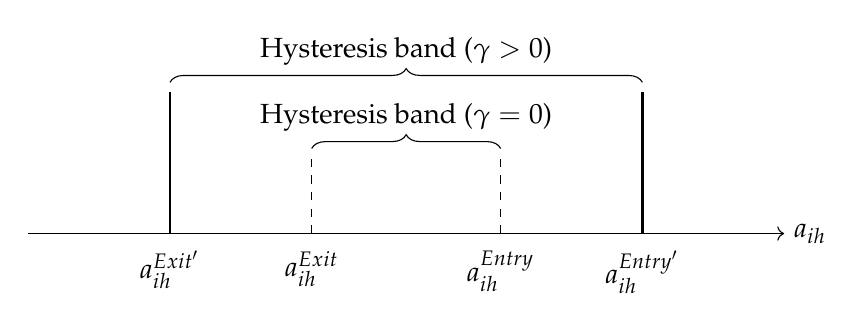
\begin{tikzpicture}[scale=1.2]

% Axis
\draw[->] (-4,0) -- (4,0) node[right] {$a_{ih}$};

% --- Baseline thresholds (gamma = 0) ---
\draw[dashed] (-1,0) -- (-1,0.8);
\node[below, yshift=-0.1cm] at (-1,0) {$a_{ih}^{Exit}$}; 

\draw[dashed] (1,0) -- (1,0.8);
\node[below, yshift=-0.1cm] at (1,0) {$a_{ih}^{Entry}$}; 

% --- Uncertainty thresholds (gamma > 0) ---
\draw[thick] (-2.5,0) -- (-2.5,1.5);
\node[below, yshift=-0.1cm] at (-2.5,0) {$a_{ih}^{Exit'}$}; 

\draw[thick] (2.5,0) -- (2.5,1.5);
\node[below, yshift=-0.1cm] at (2.5,0) {$a_{ih}^{Entry'}$}; 

% --- Braces above the axis ---
% For gamma = 0 (Lower brace, close to the axis)
\draw[decorate,decoration={brace,amplitude=5pt}]
(-1,0.9) -- (1,0.9)
node[midway,yshift=0.4cm] {Hysteresis band ($\gamma=0$)};

% For gamma > 0 (Upper brace)
\draw[decorate,decoration={brace,amplitude=5pt}]
(-2.5,1.6) -- (2.5,1.6)
node[midway,yshift=0.4cm] {Hysteresis band ($\gamma>0$)};

\end{tikzpicture}
\caption{Uncertainty widens the hysteresis band}\label{fig:band}
\end{figure}

\begin{description}
    \item[Hypothesis] \textit{The Brexit referendum reduces expected profitability and increases policy uncertainty. Under investment irreversibility arising from sunk entry and exit costs, uncertainty raises the option value of waiting and lowers the exit threshold for incumbent firms. As a result, affiliate exit responds substantially less than new entry.}
\end{description}



The combination of lower expected profitability and higher uncertainty expands the inaction region, thereby amplifying the asymmetry between entry and exit. A higher probability of deterioration ($\gamma > 0$) widens the hysteresis band by simultaneously raising the entry threshold and lowering the exit threshold. This asymmetric effect---driven by the interplay between sunk costs and policy uncertainty---predicts that the Brexit referendum reduced new Japanese FDI into the UK without triggering a proportional wave of affiliate exits.


Our model focuses on parent firm decision-making regarding foreign affiliate operations. In the following sections, we test these predictions using affiliate-level data for two reasons. First, our data availability at the affiliate level provides the granular information necessary to examine Brexit's differential impacts across affiliates with varying ownership ratios within the same parent firm. Second, while strategic decisions about market entry and exit ultimately originate with the parent firm, these decisions are implemented and manifested at the affiliate level, making affiliate-level data the most appropriate unit of analysis for testing our theoretical predictions.




\section{Data and preliminary analysis \label{sec:data}}
\subsection{The Overseas Japanese Companies Data}

This study employs the frequently used Toyo Keizai Inc.'s Overseas Japanese Companies Data (hereafter, OJC data) (e.g., recently, among others, \citealt{Bederbos2021, cieslik2022brexit}). The OJC data contains basic information on Japanese parent firms' foreign affiliates. Importantly for this study, the OJC provides a detailed analysis of each affiliate's location and Japanese parent firms' ownership percentages.\footnote{See the following page for a more detailed description of the data: \url{https://biz.toyokeizai.net/en/data/service/detail/id=860}.} The OJC data is the best available data for the analysis of exits, as it is more complete than similar government databases with respect to the number of observations and foreign affiliate-specific information. 
For this study, we combine biennial OJC survey data from 2010--2014 with annual OJC data between 2016 and 2020.\footnote{In particular, we use eight OJC surveys, including 2010, 2012, 2014, and 2016--2020.} For each affiliate, the OJC provides the data of establishment, location, total capital, employment, and parent ownership information.\footnote{The capital is recorded in various currencies. It prevents us from using the capital data in our analysis.} 


The annual OJC surveys provide the list of operating Japanese affiliates in each host country; affiliate exits are not specifically identified. Therefore, to determine an exit, we compare successive OJC surveys to determine whether an affiliate is listed in both. When an affiliate is no longer listed in the OJC, it is considered having exited the host country.\footnote{For completeness, we ensure that there is not a survey error by examining subsequent OJC surveys to confirm exit.} Since the OJC survey takes place the year prior to its release (e.g., the OJC survey released in 1992 occurred in fall 1991), we use the year prior to the survey as the affiliate exit date. 

Similarly, we can determine parent divestiture by examining the annual affiliate ownership data. As the OJC provides the ownership percentage of each affiliate parent, changes in ownership can easily be identified. For the purposes of this paper, affiliate divestiture is identified when the main Japanese owner reduces its affiliate ownership percentage. In this way, we can identify Japanese parents pulling equity out of the host country, even though the affiliate continues to exist.\footnote{Our choice of measuring divestment through equity ownership reduction is consistent with previous literature on this, including \cite{unctad2016}, \cite{javorcik2009}, and \cite{BelderbosZou2009}.} 


\subsection{Preliminary analysis}

%%%%%%%%%%%%%%%%%%%%%%%%%%%%%%%%%%%%%%%%%%%%%%%%%%%%%%%%%%%%%%%%%%%

\begin{figure}[ht]
\begin{center}
  \begin{minipage}[b]{0.45\linewidth}
    \centering
    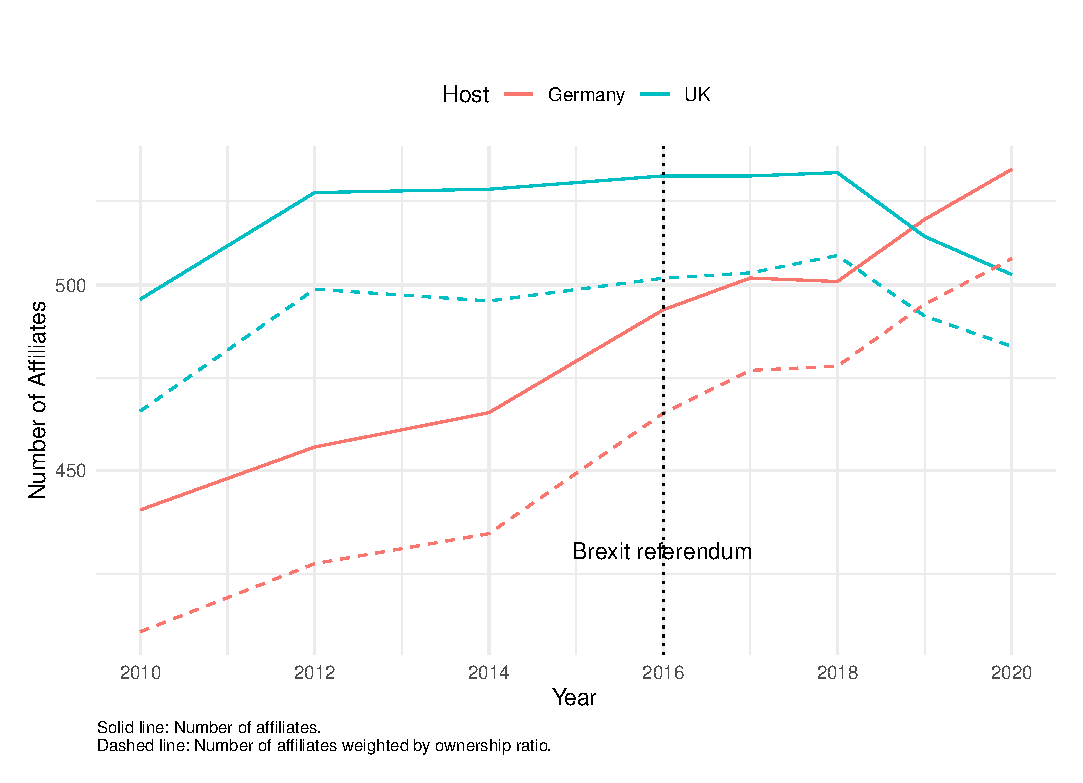
\includegraphics[keepaspectratio, scale=0.45]{Fig1a-N-WN.eps}
    \subcaption{UK and Germany}
  \end{minipage} % Do not add the empty line below.
  \begin{minipage}[b]{0.45\linewidth}
    \centering
    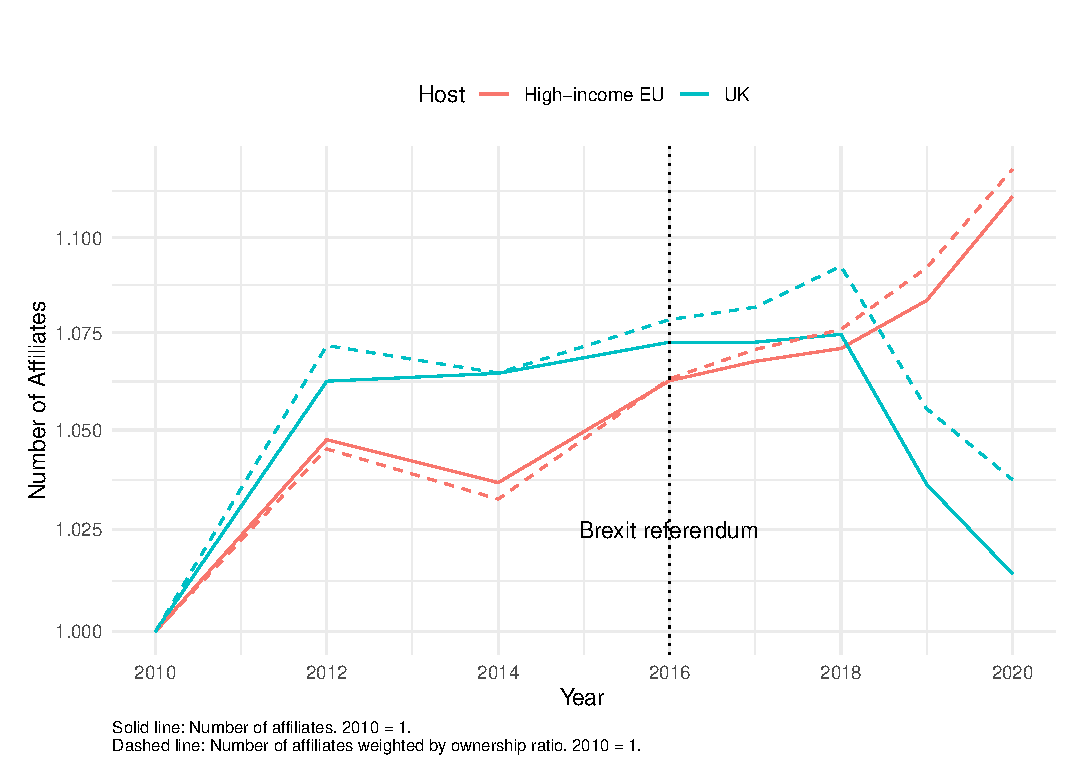
\includegraphics[keepaspectratio, scale=0.45]{Fig1b-N-EU-GBR.eps}
    \subcaption{UK and High-income EU}
  \end{minipage}
  
  \caption{Number of Japanese affiliates}
    \label{fig:GBR_DEU}

\end{center}

\vspace{0.3cm}
\footnotesize
\emph{Source:} Authors' compilation based on Toyo Keizai's OJC data.

\emph{Notes:} In both Panels, blue lines represents the values in the UK, while the red lines represents those in the comparison countries. The solid lines show the number of affiliates, while dashed lines show the number of affiliates weighted by Japanese ownership ratio. The values in Panel (b) is normalized to set the 2010 value to one. 
\end{figure}
% Des02_country_level.Rmd
%%%%%%%%%%%%%%%%%%%%%%%%%%%%%%%%%%%%%%%%%%%%%%%%%%%%%%%%%%%%%%%%%%%

The OJC data provides us with several interesting insights into Japanese FDI in the UK. First, as Panel (a) of Figure \ref{fig:GBR_DEU} indicates, there exists a leveling-off of the number of Japanese affiliates operating in the UK starting well before the Brexit referendum. As a comparison, this occurs simultaneously with increased investment into Germany (among other EU hosts) both in the total number of affiliates and affiliates weighted by Japanese ownership percentage. A decline in the number of UK-based affiliates does begin post-Brexit, while German-based affiliate numbers increase. 
Panel (b) shows a similar tendency when comparing the UK with other high-income EU countries (see Appendix Table \ref{tab:country-list} for the list of countries). Namely, in the UK, the number of affiliates dropped after the Brexit referendum. In contrast, in the other high-income EU countries, the number of affiliates continued to grow.
 
While informative, and supporting the notion that Japanese FDI is reduced post-Brexit, Figure \ref{fig:GBR_DEU} cannot tell us anything about why Japanese investment in the UK is lower.  We leave that to Figure \ref{fig:number}, which highlights Japanese exits and new entry into the UK.  Pre-Brexit, the number of new affiliates established in the UK approximately equaled UK exits, yielding the leveling-off of affiliate totals noted in Figure \ref{fig:GBR_DEU}. Exit and entry are much greater than in the other high-income EU countries, in part representing the large share of Japanese FDI that went into the UK relative to the rest of Europe. Importantly, note that after the decline in exits in 2016, exit from the UK quickly returned to previous levels.\footnote{This appears consistent with \cite{porto2023}, who find no short-run evidence of a decline in direct employment related to UK-based Japanese affiliates. In addition, they note the UK had experienced a declining share of European affiliates, especially between 2000--2010.} This is in contrast to new entries, which dropped for the UK to levels noted in the rest of the EU. By separating out exits and entries, it appears that the post-Brexit decline in investment into the UK is not from increased exit, but rather from significantly decreased entry, although rigorous causal analysis is still required.

%%%%%%%%%%%%%%%%%%%%%%%%%%%%%%%%
\begin{figure}[ht]
\begin{center}
  \begin{minipage}[b]{0.45\linewidth}
    \centering
    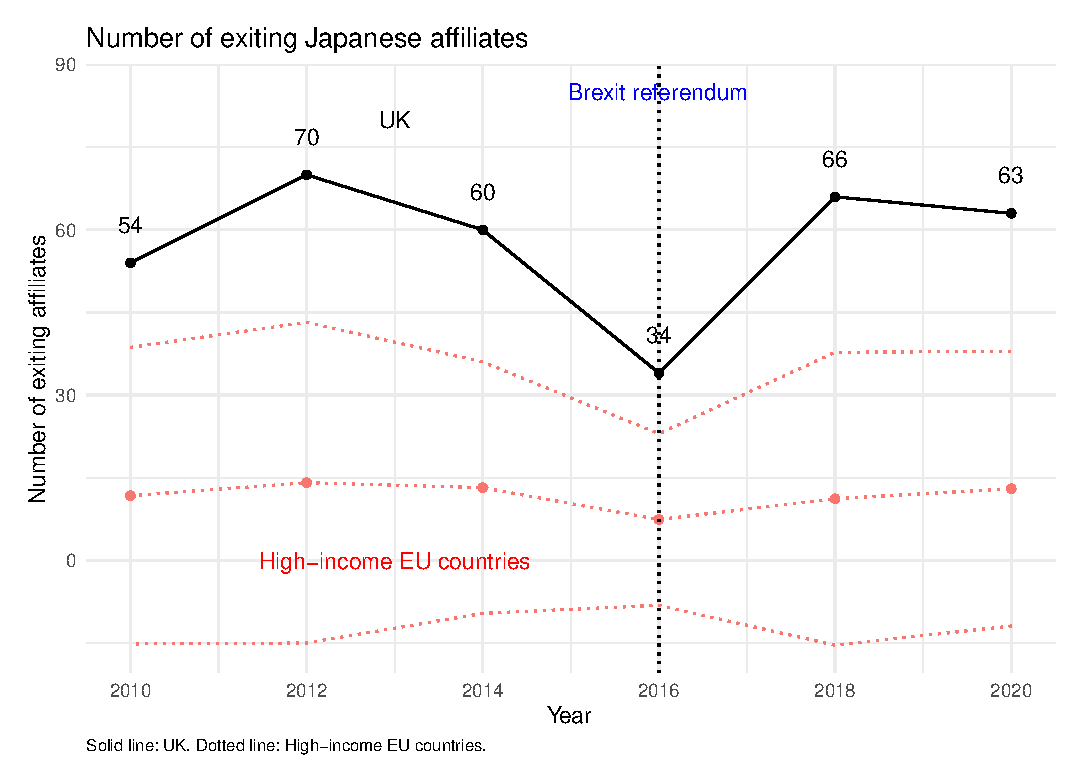
\includegraphics[keepaspectratio, scale=0.45]{Fig2a_plot_exit-compare-aff.eps}
    \subcaption{Number of exits}
  \end{minipage}
  \begin{minipage}[b]{0.45\linewidth}
    \centering
    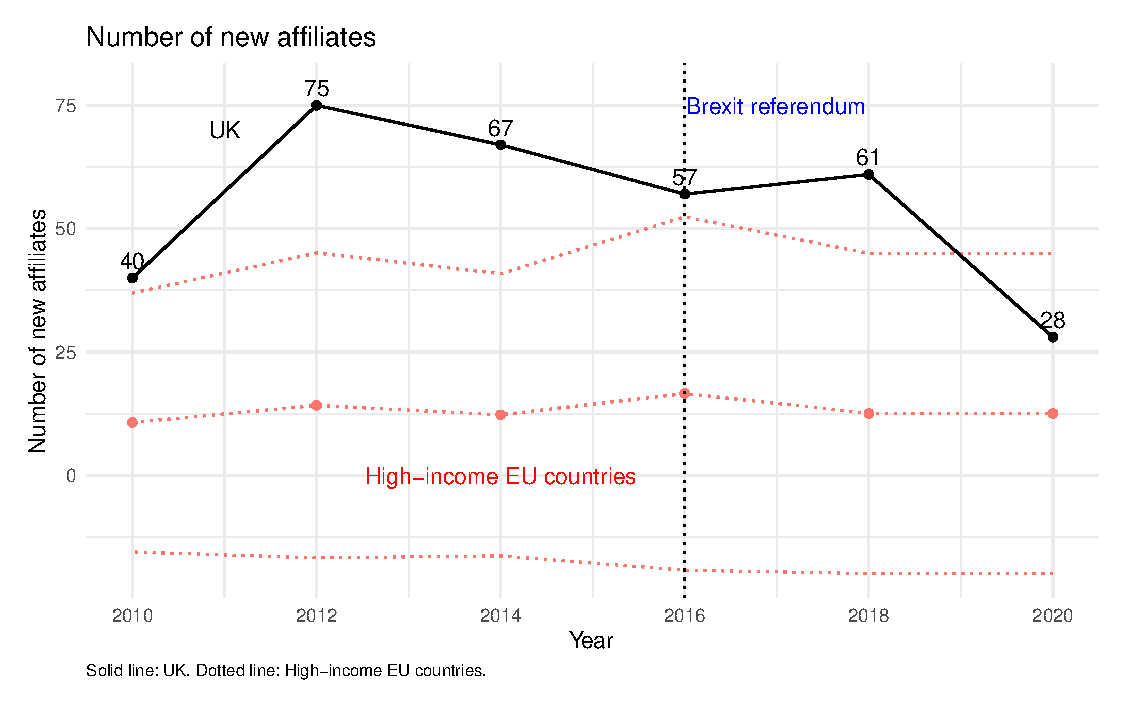
\includegraphics[keepaspectratio, scale=0.45]{Fig2b_plot_enter-aff-compare.eps}
    \subcaption{Number of new entries}
  \end{minipage}
  
  \caption{Number of Japanese affiliates}
    \label{fig:number}

\end{center}

\footnotesize
\emph{Source:} Authors' compilation based on Toyo Keizai's OJC data.\\
\emph{Note:} 
Panel (a) draws the number of Japanese affiliates exiting from a country, while Panel (b) draws those entering a country. The solid lines represent the numbers in the UK, while the dashed lines represent average numbers and confidence intervals in the other high-income EU countries.

\end{figure}
% A: Data26_brexit_firms.Rmd
% B: Data27_new_entry_another_approach.Rmd
%%%%%%%%%%%%%%%%%%%%%%%%%%%%%%%%



\section{Empirical method \label{sec:method}}


\subsection{Specification}

In order to identify the causal impacts of Brexit on affiliate exit and multinational ownership ratio, we turn to the difference-in-differences method. We use a balanced panel of Japanese affiliates in the UK and other EU countries from 2010--2020. We restrict our estimation sample to the affiliates that existed in 2010, dropping those that first appeared in the data after 2011. This is because affiliates that newly entered the UK especially after Brexit do not have comparable pre-treatment periods. In the case of estimating the exit decision, we code the exit variable as 0 when an affiliate exists in the data and 1 after it finally disappears from the data. In the case of estimating the ownership ratio, we code the ownership variable as a value between 0 and 1 when the affiliate exists in the data and 0 after it finally disappears from the data. By doing so, we can examine whether the incumbent affiliates that existed in the UK before Brexit tended to experience an exit or a reduction in the Japanese ownership ratio in the UK compared with those in other host countries.\footnote{In our online appendix, we provide simple Kaplan-Meier estimation to study Japanese exits from the UK. KM analysis enables us to assess the survival rates of different affiliate cohorts categorized by distinct characteristics (ie, affiliate location). Our results comparing UK and EU exits find the expected downward path dependence, indicating declining affiliate survival likelihood (or increased exit likelihood) as affiliates age. Importantly, results from a Mantel-Cox log-rank test indicate a p-value of 0.1, identifying no significant survival difference for Japanese affiliates in our two groups.}

The FDI-related sunk costs may produce a hysteresis effect that keeps foreign affiliates operating despite what parent firms may consider deteriorating host market effects. In light of these costs and to combat these changes, parent firms may seek to slowly reduce their foreign market exposure by divesting from their foreign affiliates and decreasing their equity ownership ratios. Our anecdotal evidence suggests that this does occur. To capture what we consider affiliate divestment more accurately, we analyze how Brexit affected the Japanese ownership ratio of UK-based foreign affiliates.
To do so, in addition to the exit variable, we use the Japanese parent firms' ownership ratio of a foreign affiliate as the outcome variable. 


Specifically, to investigate the time-varying impacts of Brexit, we conduct a dynamic analysis using the following event study specification:
\begin{equation}\label{eq:es} 
% Callaway (2022), equation (9)
% Anderson et al. (2022). https://doi.org/10.1257/pandp.20221066
Y_{i t}=\theta_{t}
+ \eta_{i}
+ \sum_{t =2010}^{2012} \beta_{t} D_{i t}
+ \sum_{t = 2016}^{2020} \beta_{t} D_{i t}
+v_{i t}
\end{equation}
where $i$ and $t \in [2010, 2020]$ index affiliate and year, respectively.
We have biennial data of 2010, 2012, and 2014 before the Brexit referendum, while we have yearly data between 2016 and 2020 after the referendum.
The outcome variable $Y_{it}$ is either the indicator variable for an affiliate exit or the Japanese ownership ratio of the affiliate.
In the case of the exit model, the outcome variable, $Y_{it}$, is a binary variable that takes a value of zero if an affiliate $i$ exists in the data in period $t$ and is equal to 1 after the affiliate exits from the host country and disappear from the data.
The binary treatment variable, $D_{i t}$, is equal to 1 for affiliate $i$ in period $t$ if an affiliate $i$ is located in the UK in period $t$ and is equal to 0 otherwise. 
The coefficients, $\beta_{t}$, are expected to capture the treatment effects of Brexit.
As it is standard practice to choose the period prior to the event as the base period, we omit $t = 2014$ from equation (\ref{eq:es}), which normalizes the estimates of $\beta_{t}$ to 0 in that year.\footnote{See, for example, \cite{frey2021}.} 
The equation (\ref{eq:es}) is often called two-way fixed effects (TWFE) model because it includes two-way fixed effects, that is affiliate fixed effects $\eta_{i}$ and year fixed effects $\theta_{t}$, in the estimation.\footnote{For the detailed description of the event study analysis and the TWFE model, see \cite{de2020two}, \cite{sun2021estimating}, \cite{callaway2023difference}, and \cite{roth2023survey} among others.}
The affiliate fixed effects absorb any time-invariant factors such as affiliate industry, affiliate type, and affiliate sizes.
Due to the high dimensional fixed effects, it becomes computationally difficult to use the logit or fractional logit models. We, therefore, use the standard alternative estimation technique (OLS) for both our exit and divestment analysis.\footnote{Given the high dimensional fixed effects, we note that our logit model regressions did not obtain convergence. In addition, it is well-known that fixed effects estimators of nonlinear panel models can be severely biased due to the incidental parameters problem \citep{fernandez2009fixed, fernandez2018fixed}.
With OLS, we can avoid these problems. In Section \ref{sec:robustness}, we follow \cite{wooldridge2021two, wooldridge2023simple}'s nonlinear DiD approach to conduct logit model estimation and confirm that our results are unchanged.
} 

% Logistic Regression and the Incidental Parameters Problem
% https://gburtch.github.io/posts/2021/03/logit-ipp/

\subsection{Identifying assumptions}
To identify the causal impacts of Brexit via equation (\ref{eq:es}), we need to assume the standard parallel trends assumption: 

\begin{align}\label{eq:pt}
\mathbb{E}\left[{Y_{i t}(0)}
-{Y_{i t^{\prime}}(0)} \mid \underbrace{D_{i}=1}_{\text{UK}} \right]
=
{\mathbb{E}\left[Y_{i t}(0)-Y_{i t^{\prime}}(0) \mid \underbrace{D_{i}=0}_{\text{Other EU}} \right]} 
\quad \textbf{for } t \neq t^{\prime} 
\end{align}
where $D_{i}$ is an indicator variable for the treated group, i.e., affiliate in the UK.\footnote{
See \cite{callaway2023difference} and \cite{roth2023survey} for a detailed explanation of the assumptions of the DiD method.
} 
Therefore, this assumption indicates that without the Brexit referendum, the average changes in the outcome of Japanese affiliates in the UK would be equal to those in other EU countries.

We also assume no anticipatory effects as follows:
\begin{align}
{Y_{i t}(0)}
=
Y_{i t}(1)  \text{ for } t < 2016 \text{ and for all } i \text { with } D_{i}=1.
\end{align}
This assumption states that the outcome before Brexit does not depend on the Brexit referendum. This assumption is validated by previous academic studies, and most of the popular press publications at the time, that indicated that a ``Leave" Brexit outcome was unlikely. For example, among others, \cite{becker_who_2017} discussed that bookmakers and pollsters predicted pre-Brexit that the ``Remain" side would win the referendum. \cite{alabrese_who_2019} also stated that the Brexit vote in the 2016 EU referendum came as a shock to many observers. We, therefore, consider the no anticipatory effects assumption is plausible.


Given the parallel trends assumption and no anticipatory effects assumption, the event study DiD specification (\ref{eq:es}) allows us to identify the average treatment effect on the treated (ATT):
\begin{align}
\tau _{2} = \mathbb{E} [ Y_{i2}(1) - Y_{i2}(0) | D_{i} = 1].
\end{align}
To validate the plausibility of the assumptions, we follow the standard practice of estimating the coefficients of the event study plot for the pre-treatment period.




\section{Baseline results \label{sec:results}}
%\subsection{Baseline event study results}\label{sec:twfe}

We conduct a dynamic analysis using the event study specification in equation (\ref{eq:es}) to estimate the time-varying impacts of Brexit on the affiliate exits and the Japanese ownership ratio of the affiliates in the UK. 
The event study coefficients are presented in Figures \ref{fig:es1} and \ref{fig:es2} with the 95\% confidence intervals.
Figure \ref{fig:es1} presents the impacts of Brexit on the affiliates' exit probability, while Figure \ref{fig:es2} shows the impacts on the Japanese ownership ratio.
Both figures use affiliates in the UK as the treated group.
In both figures, high-income EU countries are served as the comparison countries. High-income EU countries are Luxembourg, Ireland, Denmark, Netherlands, Sweden, Austria, Germany, Finland, Belgium, France, United Kingdom, and Italy.
We consider the high-income EU countries to be a more suitable comparison group than lower-income EU countries because the former tend to be more similar to the UK from the viewpoint of Japanese investors. The list of high-income EU countries is provided in the Appendix Table \ref{tab:country-list}.


%%%%%%%%%%%%%%%%%%%%%%%%%%%%%%%%%%%%%%%%%%%%%%%%%%%%%%%%
\begin{figure}[ht]
\begin{center}

    \includegraphics[keepaspectratio, scale=0.6]{Fig3-TWFE-Exit-OLS-HighEU.eps}

 \caption{Dynamic impacts of Brexit on exit probability}
    \label{fig:es1}
    
\end{center}

\footnotesize
\emph{Source:} Authors' compilation based on Toyo Keizai's OJC data.\\
\emph{Note:} The figures present the event study coefficients of equation (\ref{eq:es}) with the 95\% confidence intervals. 
The value labels indicate the estimates of the coefficients when we use the high-income EU countries as the comparison countries.
The figure draws the affiliate-level impacts of Brexit on the exit probability.
The R \texttt{fixest} package \citep{fixest} is used.

\end{figure}
% Est05_TWFE-Brexit-Affiliate-OLS.Rmd
%%%%%%%%%%%%%%%%%%%%%%%%%%%%%%%%%%%%%%%%%%%%%%%%%%%%%%%%

%%%%%%%%%%%%%%%%%%%%%%%%%%%%%%%%%%%%%%%%%%%%%%%%%%%%%%%%
\begin{figure}[ht]
\begin{center}

    \includegraphics[keepaspectratio, scale=0.6]{Fig4-TWFE-Ratio-OLS-HighEU.eps}
    
  \caption{Dynamic impacts of Brexit on ownership}
    \label{fig:es2}

\end{center}

\footnotesize
\emph{Source:} Authors' compilation based on Toyo Keizai's OJC data.\\
\emph{Note:} The figures present the event study coefficients of equation (\ref{eq:es}) with the 95\% confidence intervals. 
The value labels indicate the estimates of the coefficients. 
The figure draws the affiliate-level impacts of Brexit on the ownership ratio.
We use the high-income EU countries as the comparison countries.
The R \texttt{fixest} package \citep{fixest} is used.

\end{figure}
% Est05_TWFE-Brexit-Affiliate-OLS.Rmd
%%%%%%%%%%%%%%%%%%%%%%%%%%%%%%%%%%%%%%%%%%%%%%%%%%%%%%%%


\subsubsection*{Exit decision}

Figure \ref{fig:es1} shows the impacts of Brexit on the affiliate exit probability.
The coefficient estimates of the event study plots on the exit probability in Figure \ref{fig:es1} are relatively small, ranging from 0.9 percentage points in 2016 to 2.9 percentage points in 2020 on average. 
Furthermore, they are not statistically significant at the 5\% level.
There is a slightly upward trend in Figure \ref{fig:es1}, especially after 2019. 
However, we do not find any significant evidence that Brexit pushed Japanese affiliates out of the UK.


%we have to note that the UK faced severe pandemic impacts in those years.

We also note that the pre-treatment coefficients are not significant, suggesting that the parallel trends assumption holds.
This implies that the estimated impacts of Brexit on the affiliate exits are not biased by the pre-treatment differences between the UK and other high-income EU member countries.


\subsubsection*{Ownership ratio}

Figure \ref{fig:es2} show the impact of Brexit on Japanese multinational ownership in the UK.
We again use the high-income EU member countries as the comparison countries.
We find that the estimated impacts of Brexit on the Japanese ownership ratio are small and not statistically significant.
The estimated average impacts on the Japanese ownership ratio are insignificant and negligibly small, ranging from $-0.8$ percentage points in 2016 to $-2.9$ percentage points in 2020.
Again, we do not find any significant pre-treatment coefficients, suggesting that the parallel trends assumption holds in the ownership ratio analysis as well. 
To summarize, our baseline event study analysis indicates that Brexit had a negligible effect on both the exit probability and ownership of Japanese multinationals in the UK, consistent with our model’s prediction that hysteresis effects discourage exit and divestment.





\section{Robustness checks}\label{sec:robustness}

\subsection{Extended two-way fixed effects model}\label{sec:etwfe}

As a robustness check, we employ \cite{wooldridge2021two}'s extended two-way fixed effects (ETWFE) model to estimate the post-treatment impacts of Brexit on the affiliate exits and the Japanese ownership ratio of the affiliates in the UK.
The ETWFE model is an extended version of the TWFE model that estimates the post-treatment coefficients only.
It is robust to the heterogeneous impacts of Brexit on the affiliate exits and the Japanese ownership ratio of the affiliates in the UK.
The ETWFE model is specified as follows:
% Callaway (2023), equation (8)
\begin{align}\label{eq:ETWFE}
Y_{i t}=
\eta_{i}
+
\theta_{t}
+
\sum_{t=2016}^{2020} 
\beta_{t} 
\mathbf{1}\left\{D_{i}=1, t=q \right\}
+
v_{i t}
\end{align}
where $\eta_{i}$ and $\theta_{t}$ are affiliate and year fixed effects.
$D_{i}$ takes a value of one if an affiliate $i$ locates in the UK.
The calendar year, $q$, ranges between 2016 and 2020, namely, the post-treatment period.
The indicator variable, $\mathbf{1}\left\{D_{i}=1, t=q\right\}$, equals to one if an affiliate $i$ locates in the UK and year is $h$. 
Therefore, $\mathbf{1}\left\{D_{i}=1, t=q\right\}$ indicates the post-treatment interaction terms.

The major difference between TWFE (\ref{eq:es}) and ETWFE (\ref{eq:ETWFE}) specifications is that ETWFE only estimates post-treatment coefficients.
In other words, the ETWFE model does not estimate pre-treatment coefficients. 
Assuming that parallel trends hold in all pre-treatment periods, the ETWFE model omits to estimate parameters in pre-treatment periods and thus can produce more efficient estimates than the TWFE model if the assumption holds.
On the flip side, the TWFE model tends to produce more robust estimates in the sense that violations of parallel trends in pre-treatment periods do not lead to biased estimates of treatment effect parameters in post-treatment periods.\footnote{See \cite{callaway2023difference} for more detailed discussion.}



\cite{wooldridge2021two} shows that we can use the treatment group indicator variable instead of unit fixed effects in the ETWFE model because both result in equivalent coefficient estimates of time-varying treatment variables.\footnote{See \cite{wooldridge2021two}'s corollary 5.1 for more precise statement.}
Therefore, we can estimate the ETWFE model by using the treatment group indicator variable, $D_{i t}$, instead of the full set of affiliate fixed effects, $\eta_{i}$.
This greatly reduces the computational burden of the estimation.


Table \ref{tab:Table-ETWFE-OLS} shows the estimation result of the ETWFE model.\footnote{We used \cite{etwfe}'s R package \texttt{etwfe}.} 
The first two columns (1) and (2) present the results of the exit probability, while the last two columns (3) and (4) show the results of the ownership ratio.
The first and the third columns (1) and (3) use high-income EU member countries as comparison countries, while the second and the fourth columns (2) and (4) use all other EU member countries as comparison countries.
Table \ref{tab:Table-ETWFE-OLS} shows estimated coefficients of the post-treatment interaction terms of five years between 2016 and 2020. 
The estimated coefficients of the ETWFE model are quite similar to those of the TWFE model in the previous section.
The post-treatment interaction terms are not significant in all specifications at the conventional levels, indicating that the impacts of Brexit on the exit probability and the ownership ratio are not significant regardless of comparison countries. 
In sum, the results from the ETWFE model are consistent with those from the TWFE model, indicating that, as our model predicts, the impacts of Brexit on affiliate exits and the Japanese ownership ratio in UK affiliates are negligible.


%%%%%%%%%%%%%%%%%%%%%%%%%%%%%%%%
{\renewcommand\normalsize{\scriptsize}%
\normalsize 
\begin{table}[ht]
\centering
\caption{\label{tab:Table-ETWFE-OLS}Impacts of Brexit (ETWFE model, OLS)}
\centering
\begin{threeparttable}
\begin{tabular}[t]{lcccc}
\toprule
\multicolumn{1}{c}{ } & \multicolumn{2}{c}{Exit probability} & \multicolumn{2}{c}{Ownership ratio} \\
\cmidrule(l{3pt}r{3pt}){2-3} \cmidrule(l{3pt}r{3pt}){4-5}
\multicolumn{1}{c}{ } & \multicolumn{1}{c}{(1)} & \multicolumn{1}{c}{(2)} & \multicolumn{1}{c}{(3)} & \multicolumn{1}{c}{(4)} \\
\cmidrule(l{3pt}r{3pt}){2-2} \cmidrule(l{3pt}r{3pt}){3-3} \cmidrule(l{3pt}r{3pt}){4-4} \cmidrule(l{3pt}r{3pt}){5-5}
  & High income EU & EU & High income EU  & EU \\
\midrule
UK × Year 2016 & 0.010 & 0.006 & -0.008 & -0.006\\
 & (0.026) & (0.023) & (0.026) & (0.022)\\
UK × Year 2017 & 0.013 & 0.010 & -0.011 & -0.012\\
 & (0.031) & (0.026) & (0.030) & (0.025)\\
UK × Year 2018 & 0.006 & 0.002 & -0.008 & -0.008\\
 & (0.028) & (0.025) & (0.028) & (0.024)\\
UK × Year 2019 & 0.027 & 0.022 & -0.029 & -0.027\\
 & (0.029) & (0.026) & (0.028) & (0.024)\\
UK × Year 2020 & 0.030 & 0.025 & -0.031 & -0.030\\
 & (0.032) & (0.028) & (0.029) & (0.025)\\
\midrule
Num.Obs. & 13552 & 15424 & 13462 & 15319\\
Group Fixed-Effects & Yes & Yes & Yes & Yes\\
Year Fixed-Effects & Yes & Yes & Yes & Yes\\
R2 & 0.080 & 0.080 & 0.063 & 0.063\\
\bottomrule
\multicolumn{5}{l}{\rule{0pt}{1em}* p $<$ 0.05, ** p $<$ 0.01, *** p $<$ 0.001}\\
\multicolumn{5}{l}{\rule{0pt}{1em}}\\
\end{tabular}
\begin{tablenotes}
\item \textit{Note: } 
\item Marginal effects from \cite{wooldridge2021two}'s extended two-way fixed effects (ETWFE) model are reported in the table. Standard errors are clustered at the country level and presented in parentheses. The data are affiliate-level balanced panel data from the OJC data. The estimation uses data from 2010 to 2021, with the post-treatment period defined as 2016–2021. To improve computational efficiency, the estimation employs group-level (i.e., country-level) fixed effects instead of unit-level (i.e., affiliate-level) fixed effects. This estimation strategy follows \cite{wooldridge2021two}, which demonstrates the equivalence of group- and unit-level fixed effects in linear models. The R package `etwfe` is used for implementation.
\end{tablenotes}
\end{threeparttable}
\end{table}

}
% Est05_TWFE-Brexit-Affiliate-OLS.Rmd
%%%%%%%%%%%%%%%%%%%%%%%%%%%%%%%%




\subsubsection*{Controls}

As \cite{wooldridge2021two} discussed, the ETWFE model allows the policy effects to change with time constant controls $\mathbf{x}_{i}$.\footnote{See equation (5.15) of \cite{wooldridge2021two}.} 
By using the controls, we can relax the parallel trends assumption so that the parallel trends assumption holds only conditional on the controls. 
Under this conditional parallel trends assumption, the ETWFE model can identify the ATT.

Specifically, we extend the ETWFE model (\ref{eq:ETWFE}) by including the controls $\mathbf{x}_{i}$ as follows: 
\begin{equation} \label{eq:ETWFE2} % Wooldridge (2021) (5.15)
\begin{array}{l}
Y_{i t}=
\eta_{i}
+
\theta_{t}
+
\sum_{t=2016}^{2020} 
\beta_{t}
\mathbf{1}\left\{D_{i}=1, t=q\right\} \\
+
\sum_{t=2016}^{2020} 
\mathbf{1}\left\{D_{i}=1, t=q\right\} 
\cdot\left(\mathbf{x}_{i}-\boldsymbol{\mu}_{1}\right)
\boldsymbol{\gamma}_{t}
\\
+
\sum_{t=2016}^{2020} 
\mathbf{1}\left\{t=q\right\} 
\cdot \mathbf{x}_{i}
\boldsymbol{\delta}_{t}
+ v_{i t}
\end{array}
\end{equation} 
where 
$\boldsymbol{\mu}_{1}$ is the average of controls among the treated affiliates and calculated as $\boldsymbol{\mu}_{1}=\overline{\mathbf{x}}_{1}=N_{1}^{-1} \sum_{i=1}^{N} D_{i} \cdot \mathbf{x}_{i}$. 
We include affiliate employment and the number of affiliates in EU countries as our controls.
Affiliate employment captures affiliate size, a key determinant of exit decisions, while the number of affiliates reflects network effects that may influence divestment, as noted by \citet{norback2015}.
\footnote{\citet{norback2015} argue that the presence of other affiliates nearby can be positively correlated with divestiture.}
We use the initial values of these controls.


When using employment data from foreign affiliates, we encountered missing values that required imputation.
We employed two imputation approaches. The first is the \textit{mean imputation method}, which replaces missing values of affiliate employment with the country-year average.  
The second is the \textit{multiple imputation method}, implemented via Predictive Mean Matching (PMM) using the \texttt{mice} package in R.\footnote{\cite{hayati2015rise} describe the multiple imputation method.}

Our multiple imputation procedure generated five imputed datasets ($m=5$), based on a predefined predictor matrix that included the number of Japanese parent firms, the Japanese ownership ratio, the number of affiliates in Europe, and the number of years since establishment. To ensure convergence, we ran 50 iterations of the algorithm.
The PMM procedure consists of several steps. First, we fit regression models for affiliate employment using the specified predictors. At each iteration, we draw parameter values from their posterior distributions and calculate predicted values for both complete and incomplete cases.  
For each missing observation, we identify a set of donor cases with predicted values closest to that of the incomplete case and randomly select one donor to impute the missing value using its observed outcome.  
This process is repeated across all 50 iterations, resulting in five completed datasets that reflect both parameter uncertainty and residual variability.  


Using the imputed data, we estimated the impact of the Brexit using the ETWFE model (\ref{eq:ETWFE2}) with controls.
For multiple imputation, we fitted the ETWFE model to each of the five imputed datasets, generating five separate estimates. These estimates were then combined using Rubin’s rules, which account for both within-imputation and between-imputation variance, to produce a single, robust estimate per event time.



Figure~\ref{fig:imputed} presents event study plots based on two imputation methods. The solid line shows the results from mean imputation, while the dashed line shows those from multiple imputation. The plots indicate that the estimated impact of Brexit on exit probability is statistically insignificant at conventional levels, regardless of the imputation method. These findings are consistent in both magnitude and statistical significance with those reported in Table~\ref{tab:Table-ETWFE-OLS} and Figure~\ref{fig:es1}, and further support our prediction that hysteresis discourages exit.



%%%%%%%%%%%%%%%%%%%%%%%%%%%%%%%%%%%%%%%%%%%%%%%%%%%%%%%%%
\begin{figure}[ht]
  \begin{center}
    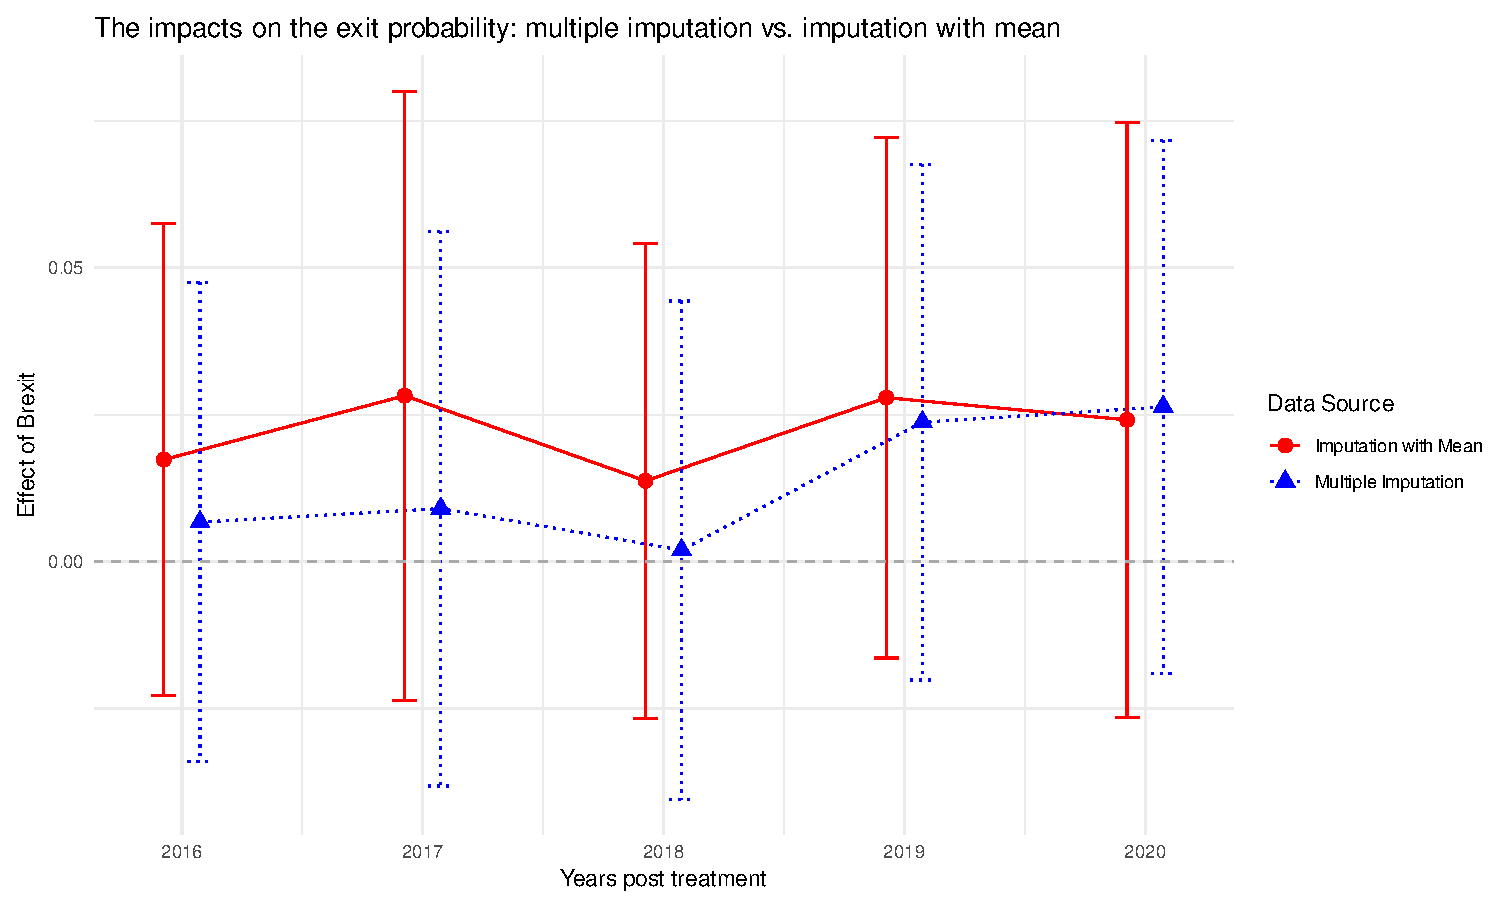
\includegraphics[width=0.8\linewidth]{Fig5-Imputation.eps}
    \caption{Brexit's impact on exit probability (multiple vs. mean imputation)}
    \label{fig:imputed}

  \end{center}

    \footnotesize
    \emph{Source:} Authors' compilation based on Toyo Keizai's OJC data.\\
    \emph{Note:} The figures present the event study coefficients of equation (\ref{eq:ETWFE2}) with the 95\% confidence intervals. 
    The figure draws the affiliate-level impacts of Brexit on the exit probability.
    The solid line represents the results of the imputation with mean, while the dashed line represents those of the multiple imputation method.
    We use the high-income EU countries as the comparison countries.
    The R \texttt{etwfe} package is used.
\end{figure}
% Est12_ETWFE-Brexit-Affiliate-OLS-MICE.Rmd
%%%%%%%%%%%%%%%%%%%%%%%%%%%%%%%%%%%%%%%%%%%%%%%%%%%%%%%%%



\subsection{Nonlinear DiD}\label{logit}

So far, we have used the linear DiD models to estimate the impacts of Brexit on the exit probability of Japanese affiliates in the UK.
\cite{wooldridge2023simple} recommends comparing the linear DiD estimates to the ATT estimates from a nonlinear method when applying DiD to limited dependent variables.
Following his recommendation, in this subsection, we estimate the logit model to examine the robustness of the results.
The logit model is a non-linear model that is often used to estimate the probability of a binary outcome. 
However, the logit model with high dimensional fixed effects is computationally challenging and can be biased due to the incidental parameters problem \citep{fernandez2009fixed, fernandez2018fixed}.
\cite{wooldridge2021two, wooldridge2023simple} show that the logit model can be used in the framework of the ETWFE model. 
As in the linear case, we employ the ETWFE model with group-level fixed effects instead of those with the unit-level fixed effects in our nonlinear specification.
By doing so, we can avoid the computational burden and obtain convergence.\footnote{When we use the logit model to estimate the ATTs, we need to specify parallel trends assumption that is analogous to the linear case's one (\ref{eq:pt}). First, we assume that $Y_{t}(0)$ is binary and generated by a latent variable, $Y_{t}^{*}(0)$, as follows:
$$
Y_{t}(0)=1\left[Y_{t}^{*}(0)>0\right]
$$
where $1[\cdot]$ is the indicator function.
Following \cite{wooldridge2023simple}, we define the latent variable $Y_{t}^{*}(0)$ by the following linear model:
\begin{equation}
Y_{t}^{*}(0)=\alpha + \beta D +\gamma_{t}+U_{t}
\end{equation}
where $U_{t}$ is continuous and independent of $D$ and identically distributed with CDF $F(\cdot)$. Then, we assume that the linear parallel trends assumption holds for the underlying latent variable as follows:
\begin{equation}
  E\left[Y_{t}^{*}(0) \mid D\right]=\alpha+\beta D+\gamma_{t}.
\end{equation}
It corresponds to the equations (2.9) and (2.10) of \cite{wooldridge2023simple}.
More detailed and general description are given in the Section 3 of \cite{wooldridge2023simple}.
In our case, this parallel trends assumption implies that the average changes in the latent variable of Japanese affiliates in the UK would be equal to those in other EU countries without the Brexit referendum.
Following \cite{wooldridge2023simple}, we test parallel trends assumption via the pre-trend test using the untreated observations. 
The cluster-robust Wald test could not reject the null that the pre-treatment coefficients equal zero (p-value $= 0.995$).
% 13c_TWFE-Brexit-Affiliate-Logit.Rmd
We, therefore, consider the parallel trends assumption is likely to hold in our nonlinear case.
}

The estimation results of the logit model are presented in Figure \ref{fig:logit}. 
The figure shows the event study coefficients of the ETWFE model with the 95\% confidence intervals.
Basically, the results of the logit model are consistent with those of the OLS model.
The estimated impacts of Brexit on the exit probability are not significant at the conventional levels.
Furthermore, the estimated ATTs are close to those of the baseline model and the linear ETWFE model. 
The results suggest that the impacts of Brexit on the affiliate exits are limited and negligible regardless of the model specification. 

%%%%%%%%%%%%%%%%%%%%%%%%%%%%%%%%%%%%%%%%%%%%%%%%%%%%%%%%
\begin{figure}[ht]
\begin{center}

    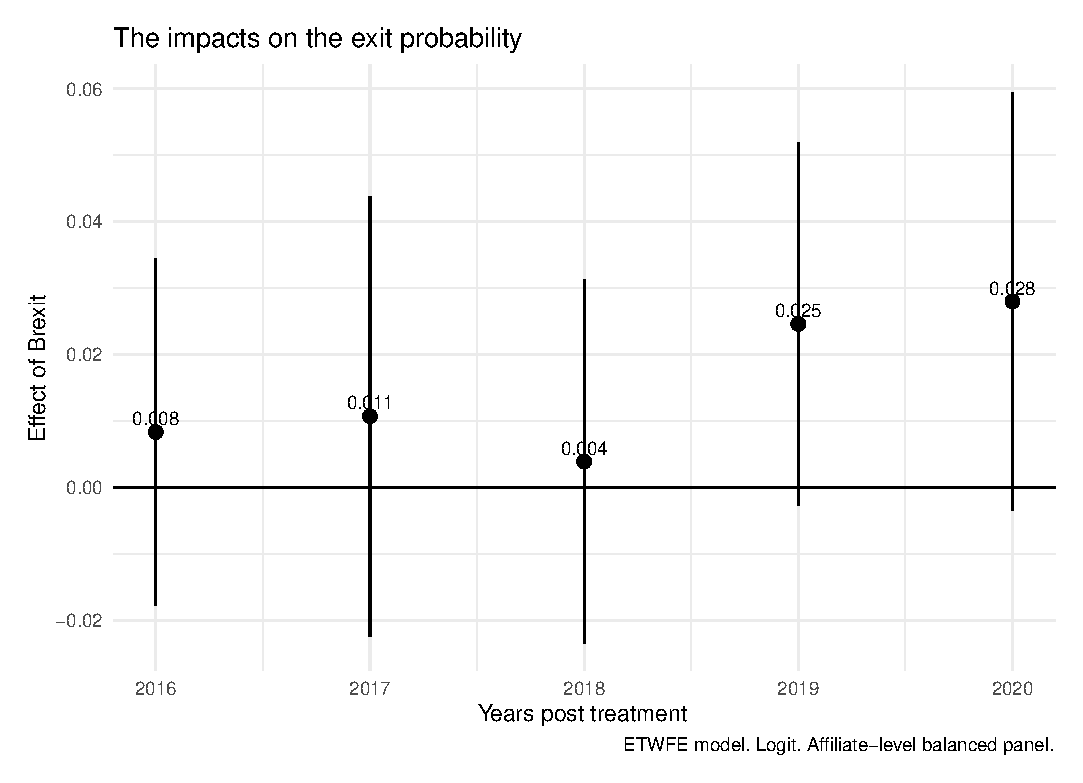
\includegraphics[keepaspectratio, scale=0.6]{Fig6-ETWFE-exit-logit.eps}

 \caption{Dynamic Impacts of Brexit on Exit Probability (Nonlinear DiD)}
    \label{fig:logit}
    
\end{center}

\footnotesize
\emph{Source:} Authors' compilation based on Toyo Keizai's OJC data.\\
\emph{Note:} The figures present the event study coefficients of \cite{wooldridge2023simple}'s extended two-way fixed effects (ETWFE) model with the 95\% confidence intervals. 
The logit model is employed.
The figure draws the affiliate-level impacts of Brexit on the exit probability.
The R \texttt{etwfe} package is used.

\end{figure}
% Est06_TWFE-Brexit-Affiliate-Logit.Rmd
%%%%%%%%%%%%%%%%%%%%%%%%%%%%%%%%%%%%%%%%%%%%%%%%%%%%%%%%


\subsection{Synthetic DiD}

So far, we have relied on the DiD methods to estimate the impact of Brexit.
As a robustness check, in this section, we conduct an analysis based on the synthetic difference-in-differences (SDiD) method.
In general, the DiD method is applied when a substantial number of units are exposed to a policy, and researchers hope to make the parallel trends assumption, which implies that selection effects can be adequately controlled by accounting for unit-specific and time-specific additional fixed effects.
However, in the case that policy changes are not random across units or periods, the parallel trends assumption may not be reliable.

\cite{arkhangelsky2021synthetic} proposed the SDiD method that combines the appealing features of both DiD and the synthetic control (SC). 
In contrast to DiD, the SC method attempts to compensate for the lack of parallel trends by re-weighting units to match pre-exposure trends.
The SC method is introduced in settings where only one (or a few) units are exposed and not applied to large panels.
Like SC, the SDiD method matches units by weighting the pre-exposure trends, thereby reducing reliance on the parallel trends assumption. 
Similar to DiD, the SDiD method allows for valid inference in large panels.


In SDiD, we include both affiliate fixed effects ($\eta_{i}$) and year fixed effects ($\theta_{t}$) into the model, as in the basic two-way fixed effects regression.
In addition, we introduce two weights into the model. 
We find the affiliate weights ($\hat{\omega}_{i}$) that align pre-exposure trends in the outcome of unexposed units with those for the exposed units.
We also look for the year weights ($\hat{\lambda}_{t}$) that balance pre-exposure time periods with post-exposure ones.\footnote{
% Guido Imbens. "CAUSAL INFERENCE WITH PANEL DATA: NEW METHODS AND REMAINING CHALLENGES"
The affiliate weights ($\hat{\omega}_{i}$) and the time weights ($\hat{\lambda}_{t}$) are obtained as follows.
\begin{equation}
\hat{\omega} \equiv\arg \min _{\omega \geq 0, \sum_{i=1}^{N-1} \omega_{i}=1} \sum_{t=1}^{T-1}\left(Y_{N t}-\sum_{j=1}^{N-1} \omega_{j} Y_{j t}\right)^{2},
\qquad
\hat{\lambda} \equiv \arg \min _{\lambda \geq 0, \sum_{t=1}^{T-1} \lambda_{t}=1} \sum_{i=1}^{N-1}\left(Y_{i T}-\sum_{t=1}^{T-1} \lambda_{j} Y_{j t}\right)^{2}.
\end{equation}
See equations (4) and (6) of \cite{arkhangelsky2021synthetic} for more details.
}
Using these two weights, equation (\ref{eq:SDiD}) minimizes the residual sum of squares so that the average causal effect of exposure ($\tau$) is estimated.


\begin{align} \label{eq:SDiD}
\left(\hat{\tau}, \hat{\mu}, \hat{\eta}, \hat{\theta}\right)
=
\underset{\tau, \mu, \eta, \theta}{\arg \min }
\left\{\sum_{i=1}^{N} \sum_{t=2010}^{T}
\left(Y_{i t}-\mu-\eta_{i}-\theta_{t}
-W_{i t} \tau \right)^{2}
\underbrace{\hat{\omega}_{i} \hat{\lambda}_{t}}_{\text{weights}}
\right\}
\end{align}
where $N$ is the number of affiliates and $T=2020$. $Y_{it}$ is the outcome variable and $\mu$ is the constant.
The Brexit dummy, $W_{it}$, takes a value of one if the host country is the UK and $t \geq 2016$ and zero otherwise.

%%%%%%%%%%%%%%%%%%%%%%%%%%%%%%%%%%%%%%%%%%%%%%%%%%%%%%%%
\begin{figure}[ht]
    \begin{minipage}{.95\linewidth}
    \begin{center}
    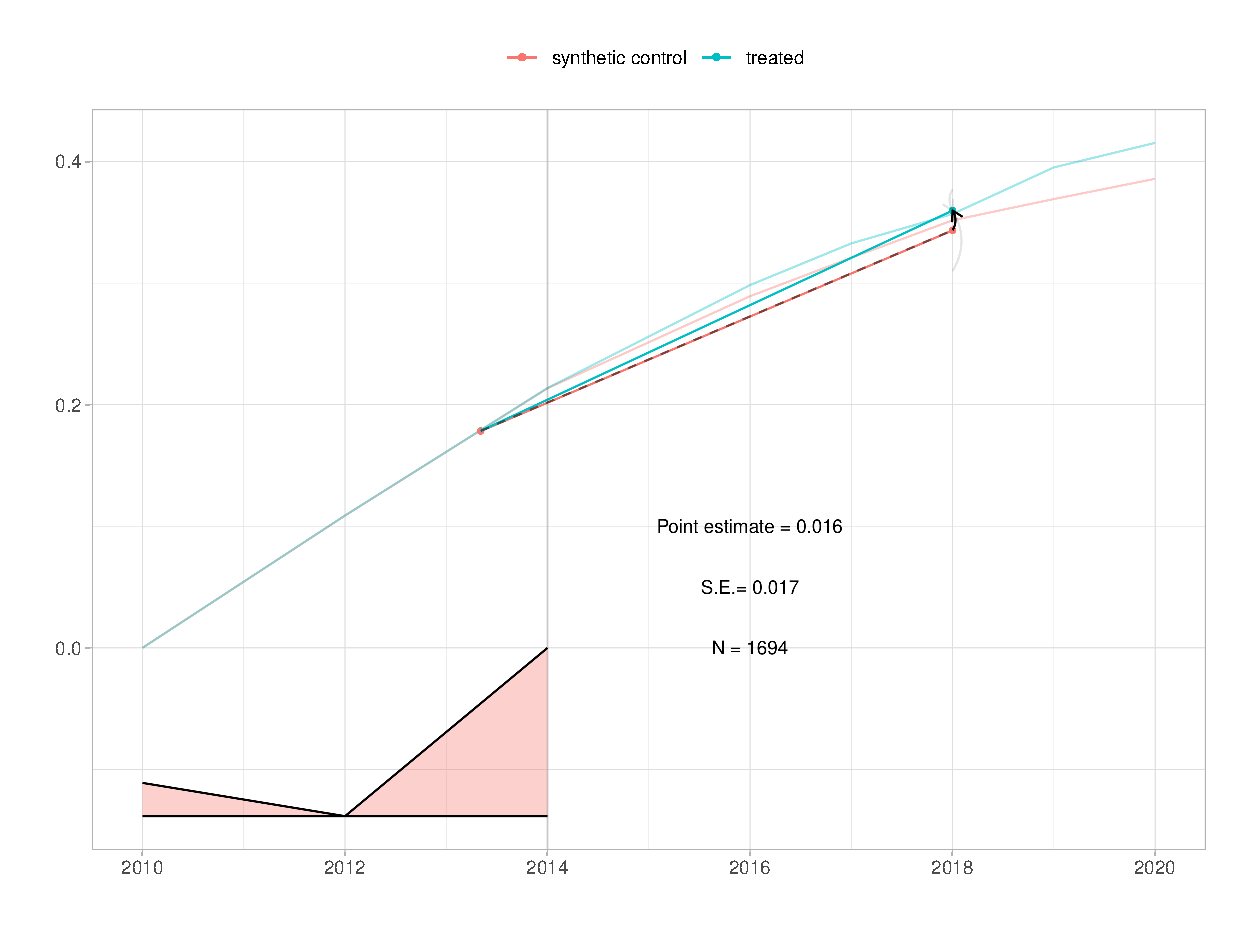
\includegraphics[width=0.7\linewidth]{Fig7-SDiD.eps}
    \caption{Brexit's Impact on Affiliate Exits (Synthetic DiD)}
    \label{fig:fig_SDiD-2}
    \end{center}

\footnotesize
\emph{Source:} Authors' compilation based on Toyo Keizai's OJC data.\\
\emph{Notes:} The figures show the results of synthetic DiD analysis based on the method of \cite{arkhangelsky2021synthetic}. 
The R \texttt{synthdid} package is used.  
We show trends in exit probability over time for Japanese affiliates in the UK and the relevant weighted average of control affiliates in other high-income EU countries, with the weights used to average pre-treatment periods shown as a shaded area at the bottom of the graphs. 
The blue lines indicate the treated group, while red line shows the control group.
The dashed line is the synthetic control.
The estimated effect is indicated by an arrow.
\end{minipage}

\end{figure}
% Est08_Brexit_SDiD_Aff.Rmd
% R failed to adequately create the Figure in EPS format. 
% Therefore, I made the Figure in PDF with R, then coverted it to EPS via online converter. https://convertio.co/pdf-eps/
%%%%%%%%%%%%%%%%%%%%%%%%%%%%%%%%%%%%%%%%%%%%%%%%%%%%%%%%

Figure \ref{fig:fig_SDiD-2} shows the results of the SDiD analysis at the affiliate level.\footnote{We used \cite{synthdid}'s \texttt{synthdid} package.} 
The blue line presents the trends in exit probability over time for Japanese affiliates in the UK and the red line presents the relevant weighted average of control affiliates in other high-income EU countries.
The weights used to average pre-treatment periods are shown as the red-shaded areas at the bottom of the graph.\footnote{The control unit weights are aggregated at country-level and reported in \ref{sec:sdid_weights}.}
The estimated effect is indicated by an arrow.
The figure shows that the trends in exit probability for Japanese affiliates in the UK and the weighted average of control affiliates in other high-income EU countries are quite similar.
The point estimate of the effect of Brexit on the exit probability is 0.016, with a standard error of 0.017.
Thus, the estimated effect of Brexit on the exit probability is negligible and insignificant, suggesting that Brexit did not have a significant impact on the exit probability of Japanese affiliates in the UK.
Overall, the results of the SDiD analysis are consistent with those of the TWFE and ETWFE models, indicating that the impacts of Brexit on the affiliate exits are limited and negligible.


\section{Identifying the mechanism \label{sec:mechanism}}
\subsection{Asset specificity}\label{sec:assetchannel}

Employing various empirical methods, we establish a robust finding: Brexit had negligible and statistically insignificant effects on Japanese FDI exits and divestitures in the UK. As outlined in our model in Section \ref{sec:Model}, the hysteresis effect of FDI significantly shapes firms' exit decisions. This effect implies that substantial sunk costs associated with FDI discourage firms from exiting, even when the host country becomes less attractive for investment. Consequently, affiliates in industries with higher asset specificity, which typically involve larger sunk costs, are expected to be less responsive to the Brexit shock.

To elucidate the mechanism behind this hysteresis effect, we investigate the heterogeneous impacts of Brexit on exit probability based on asset specificity. \cite{kermani2023asset} argue that high asset specificity is associated with less disinvestment and that the degree of asset specificity varies across industries. In our framework, we introduce asset specificity, denoted by $\rho_s \in (0, 1]$, where $\rho_s$ measures the degree to which investments in industry $s$ are sunk (i.e., non-recoverable). 

High $\rho_s$ (e.g., $\rho_s \to 1$) reflects industries with highly specific assets, such as specialized manufacturing plants, while low $\rho_s$ (e.g., $\rho_s \to 0$) characterizes industries with transferable assets, such as retail or generic office spaces. We incorporate $\rho_s$ into the incumbent's continuation condition. Following the logic of equation (\ref{eq:exit}), the condition for an incumbent firm ($FDI_{ih,t-1}=1$) to remain active in the host country is:
\begin{equation}
\pi_i(a_{ht}, \mathbf{z}_{it}) + \delta \left[ E_t \left( V_{ih,t+1} \mid FDI_{iht} = 1 \right) - E_t \left( V_{ih,t+1} \mid FDI_{iht} = 0 \right) \right] \geq -F_i^{Exit}(\rho_s),
\end{equation}
where $F_i^{Exit}(\rho_s)$ represents the effective exit cost, which increases with the degree of asset specificity $\rho_s$. 

As discussed in Section \ref{sec:Model}, Brexit reduces the current profitability $\pi_i$ and the expected future value $V_{ih,t+1}$ due to a decline in business conditions $a_{ht}$. However, for industries with high asset specificity ($\rho_s \approx 1$), the exit threshold $a_{ih}^{Exit}$ is significantly lowered (i.e., shifted to the left in Figure \ref{fig:band}). Furthermore, as shown in our uncertainty analysis, the increased probability of future deterioration ($\gamma > 0$) raises the option value of waiting, further insulating these firms from exit. In contrast, in industries with low asset specificity ($\rho_s \approx 0$), assets can be liquidated or repurposed more easily, resulting in a smaller $F_i^{Exit}$ and a higher exit threshold $a_{ih}^{Exit'}$. In these sectors, the same negative shock to $a_{ht}$ is more likely to trigger the exit condition.

This framework predicts that Brexit has minimal impact on FDI exits in high asset specificity industries due to the substantial hysteresis band, while it may significantly increase exits in low asset specificity industries where the band is narrower. To examine this, we utilize data from \cite{kermani2023asset} to categorize industries into those with low and high asset specificity. The classification procedure is detailed in Appendix \ref{sec:asset}.

We perform event study regressions for the subsamples of industries with low and high asset specificity. Figure \ref{fig:asset} presents the results of this analysis. As hypothesized, Figure \ref{fig:asset} shows that exit probabilities in low asset specificity industries (black line) rose significantly in 2019--2020, while those in high asset specificity industries (red line) remained stable. Specifically, Brexit significantly increased the exit probability in low asset specificity industries by approximately 7\% in 2019--2020 ($p < 0.05$), while it did not affect the exit probability in high asset specificity industries. These findings indicate that the hysteresis effect is stronger in industries with high asset specificity, aligning with prior studies by \cite{kermani2023asset} and \cite{kim2017asset}. Overall, our results substantiate the hypothesis that the interplay between sunk costs and policy uncertainty creates significant hysteresis, particularly when assets are highly industry-specific.


%%%%%%%%%%%%%%%%%%%%%%%%%%%%%%%%%%%%%%%%%%%%%%%%%%%%%%%%
\begin{figure}[ht]
\begin{center}

    \includegraphics[keepaspectratio, scale=0.6]{Fig8-AssetSpecificity.eps}

 \caption{Asset specificity and Brexit's dynamic impact on exit probability}
    \label{fig:asset}
    
\end{center}

\footnotesize
\emph{Source:} Authors' compilation based on Toyo Keizai's OJC data.\\
\emph{Note:} The figures present the event study coefficients of the two-way fixed effects (TWFE) model with the 95\% confidence intervals. 
The figure draws the affiliate-level impacts of Brexit on the exit probability.
The R \texttt{fixest} package is used.

\end{figure}
% Est14_TWFE-Brexit-Affiliate-OLS_Specificity.Rmd
%%%%%%%%%%%%%%%%%%%%%%%%%%%%%%%%%%%%%%%%%%%%%%%%%%%%%%%%


\subsection{The impacts on the new entry} \label{sec:entry}

So far, we have focused on the impact of Brexit on the exit behavior of incumbent Japanese affiliates in the UK. The results suggest that Brexit did not have a significant effect on the likelihood of exit, except in industries characterized by low asset specificity. We argue that this outcome may be attributed to the hysteresis effect in FDI. This effect implies that the sunk costs associated with FDI are substantial, making affiliates reluctant to exit even when the host country becomes less attractive for investment. However, while the hysteresis effect may dampen the impacts of Brexit on affiliate exit, Brexit could still exert a significant influence on the entry of new Japanese affiliates, since new entrants do not incur sunk costs until they are established, as discussed in Section~\ref{sec:Model}.

In this section, we investigate the impact of Brexit on the entry of new Japanese affiliates into the UK. While relying on the same dataset used in the preceding sections, we focus specifically on new entries. Evidence of a significant negative effect of Brexit on entry would provide further support for our hypothesis that the hysteresis effect influences the behavior of Japanese affiliates in the UK.

Figure~\ref{fig:fig_SDiD-entry} presents the results of the SDiD analysis at the industry level for new entry. It illustrates the trends in new entries of Japanese affiliates in the UK over time, compared to the weighted average of control affiliates in other high-income EU countries, also at the industry level. The weights used to compute the pre-treatment averages are shown by the shaded area at the bottom of the graph.\footnote{The control unit weights are aggregated at country-level and reported in \ref{sec:sdid_weights}.} The blue line represents the treated group, while the red line indicates the control group. The two lines closely track each other prior to the Brexit referendum, suggesting that the parallel trends assumption holds.
The dashed line depicts the synthetic control, and the estimated treatment effect is marked by an arrow in the figure. The results indicate that Brexit had a significantly negative effect on new entry, with a point estimate of $-0.145$ and a standard error of 0.052. These results are consistent with the findings of \cite{breinlich2020} and \cite{cieslik2022brexit}, and they support our theoretical prediction that Brexit would have asymmetric effects on exit and entry due to the presence of sunk costs.

%%%%%%%%%%%%%%%%%%%%%%%%%%%%%%%%%%%%%%%%%%%%%%%%%%%%%%%%
\begin{figure}[ht]
  \begin{minipage}{.95\linewidth}
  \begin{center}
  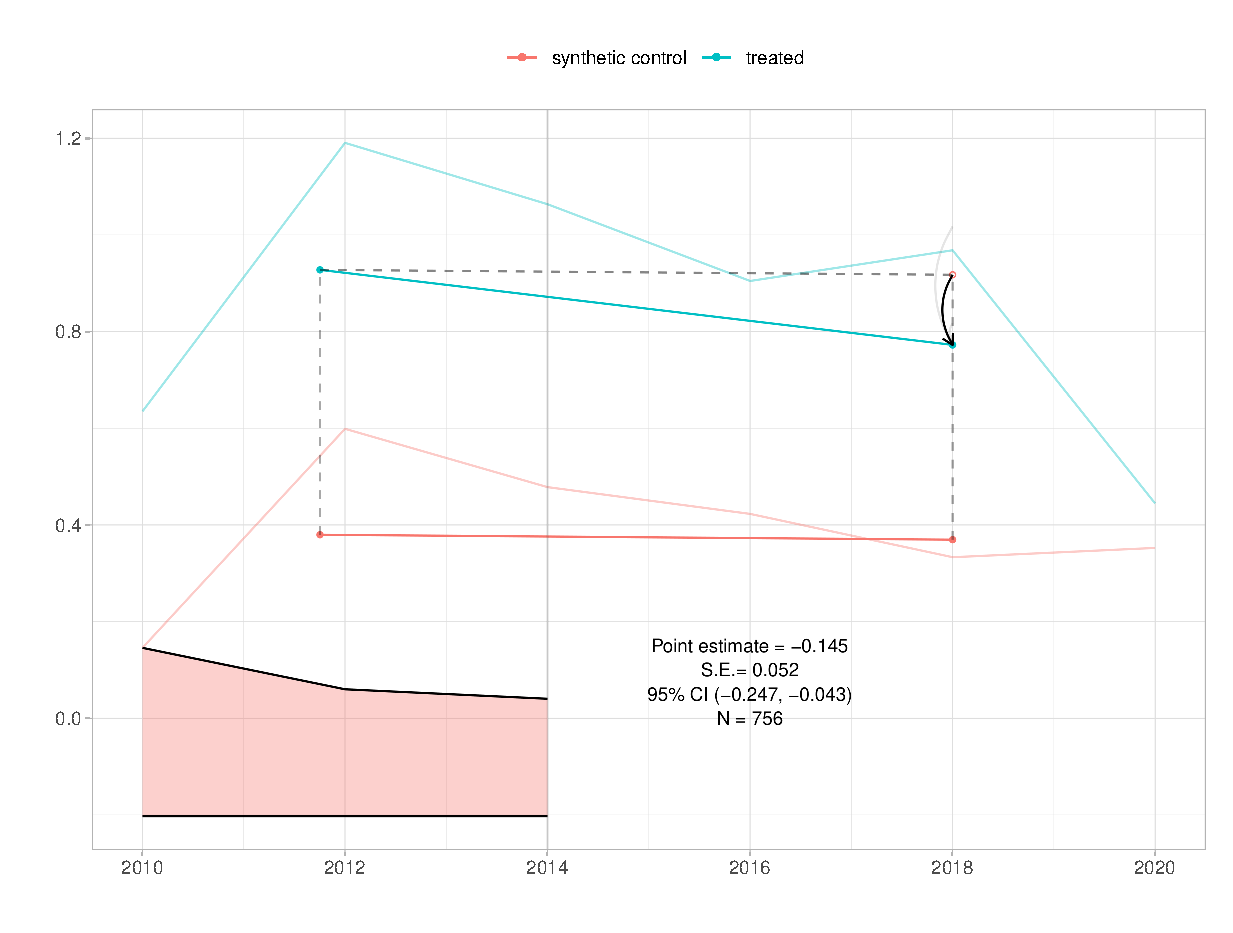
\includegraphics[width=0.7\linewidth]{Fig9-SDiD-Entry.eps}
  \caption{Brexit's Impact on New Affiliate Entries (Synthetic DiD)}
  \label{fig:fig_SDiD-entry}
  \end{center}

\footnotesize
\emph{Source:} Authors' compilation based on Toyo Keizai's OJC data.\\
\emph{Notes:} The figures show the results of synthetic DiD analysis based on the method of \cite{arkhangelsky2021synthetic}. 
The R \texttt{synthdid} package is used.  
We show trends in new entry over time for Japanese affiliates in the UK and the relevant weighted average of control affiliates in other high-income EU countries at the industry level, with the weights used to average pre-treatment periods shown as a shaded area at the bottom of the graphs. 
The blue lines indicate the treated group, while red line shows the control group.
The dashed line is the synthetic control.
The estimated effect is indicated by an arrow.
\end{minipage}

\end{figure}
% Est09_Brexit_SDiD_Entry.Rmd
% R failed to adequately create the Figure in EPS format. 
% Therefore, I made the Figure in PDF with R, then coverted it to EPS via online converter. https://convertio.co/
%%%%%%%%%%%%%%%%%%%%%%%%%%%%%%%%%%%%%%%%%%%%%%%%%%%%%%%%





\section{Conclusion\label{sec:conclusion}}

This paper presents a theoretical model incorporating sunk costs and policy uncertainty to understand affiliate exit and entry, and empirically examines the impact of Brexit on incumbent Japanese affiliates in the UK. Utilizing Toyo Keizai Inc.’s Overseas Japanese Companies Data from 2010 to 2020, we employ various difference-in-differences and synthetic difference-in-differences methods to assess the probability of exit and changes in ownership among these affiliates, compared to those in other EU countries. The results indicate no significant impact of Brexit on exits or divestment by Japanese affiliates, except in industries characterized by low asset specificity. This result aligns with our model’s prediction that hysteresis in foreign direct investment---driven jointly by high sunk costs and the option value of waiting under policy uncertainty---deters exit despite growing concerns over the UK’s diminishing market attractiveness. Specifically, our model shows that Brexit-related uncertainty ($\gamma > 0$) widens the hysteresis band by lowering the exit threshold for incumbent firms, meaning that even a negative profitability shock need not trigger exit when uncertainty is sufficiently high.

Policymakers can capitalize on hysteresis by offering targeted incentives to existing affiliates, such as tax breaks or regulatory stability, to maintain FDI stocks during policy shocks. These findings also inform future customs union exits, highlighting the need to address sunk cost barriers and manage policy uncertainty to mitigate FDI declines.

It is crucial to consider the broader context of Japanese FDI in the UK. Notably, our data show that the number of Japanese affiliates in the UK began to level off well before the Brexit referendum, accompanied by increased investment in the rest of the EU. On the one hand, the findings of this paper indicate that the ``upping sticks" phenomenon—feared by the Japanese government in 2016—did not materialize among existing affiliates. On the other hand, our analysis in Section~\ref{sec:mechanism}, along with evidence from parallel research by \cite{cieslik2022brexit}, reveals that new Japanese FDI into the UK declined significantly following the Brexit announcement. Taken together, these findings align with our model’s prediction that Brexit would have an asymmetric impact on entry and exit due to sunk costs, implying that the overall decline in Japanese investment in the UK has been driven primarily by reduced entry rather than increased exit.


Future research could extend the FDI model presented in this paper by incorporating firm heterogeneity, as in \citet{graziano2021brexit} for exporting. Investigating how firm heterogeneity interacts with the sunk cost hysteresis and option value mechanisms identified here would be a promising avenue for further study.

Research could also extend the analysis to other foreign investors in the UK to assess whether the observed hysteresis effects apply to firms from different countries. Additionally, future work might examine Brexit-related exits beyond 2020. While incorporating data from the COVID-affected years (2021, 2022, and beyond) may seem valuable, doing so would likely introduce confounding factors that obscure the specific effects of Brexit on Japanese FDI. Disentangling the impact of the pandemic would require a separate analytical approach and lies beyond the scope of the present study. Nevertheless, future work could explore the interaction between Brexit and the pandemic to better understand their combined effects on investment behavior.
Finally, the UK–Japan Comprehensive Economic Partnership Agreement, as well as trade and investment arrangements between the UK and the EU, remained uncertain during the period under study. The extent to which these agreements have helped retain Japanese affiliates in the UK remains an open question for future research.

\section*{Acknowledgments}
\noindent We are grateful to anonymous referees for their constructive comments and suggestions, which greatly improved the paper.
We also thank Tamae Kawasaki for her invaluable guidance on the imputation methods.
Tanaka acknowledges financial support from the Japan Society for the Promotion of Science (JSPS): KAKENHI Grant Number JP19K01612 and JP23K01356. The usual disclaimer applies.

\vspace{0.5cm}
\noindent
\textbf{Data availability statement}
The data that support the findings of this study are not publicly available. 
\newline
\textbf{Funding statement}
This study is partly supported by JSPS’s Grants-in-Aid for Scientific Research (No. 19K01612 and 23K01356).
\newline
\textbf{Conflict of interest disclosure}
The authors declare no conflicts of interest.

%%%%%%%%%%%%%%%%%%%%%%%%%%%%%%%%%%%%%%%%%%%%%%%%%
%\clearpage
%\begin{singlespace}
%\bibliographystyle{plainnat}
%\bibliographystyle
%\bibliographystyle{apalike}
%\bibliographystyle{aer}
%\bibliographystyle{jpe}
%\bibliographystyle{econ-econometrica}
\bibliographystyle{econ-aea}
\bibliography{brexit_ref.bib}
%\end{singlespace}
%%%%%%%%%%%%%%%%%%%%%%%%%%%%%%%%%%%%%%%%%%%%%%%%%



%%%%%%%%%%%%%%%%%%%%%%%%%%%%%%%%%%%%%%%%%%%%%%%%%
%%%%% These commands start the appendix and change the Table & Figure numbering
\newpage
\appendix
\setcounter{table}{0}
\renewcommand{\tablename}{Appendix Table}
\renewcommand{\figurename}{Figure}
\renewcommand{\thetable}{A\arabic{table}}
\setcounter{figure}{0}
\renewcommand{\thefigure}{A\arabic{figure}}
%%%%%%%%%%%%%%%%%%%%%%%%%%%%%%%%%%%%%%%%%%%%%%%%%


%\begin{appendices}

\appendix
\newpage 
\section*{Appendices}


\section{Country list}\label{country}

Table \ref{tab:country-list} reports the number of observations by host country.
We only use foreign affiliates in which Japanese parent firms own more than 10\% of the equity.
For the empirical analysis, we restrict the sample to affiliates that existed in 2010, constructing a balanced panel spanning from 2010 to 2020.
Accordingly, the number of observations for each host country in Table \ref{tab:country-list} equals the number of affiliates in 2010 multiplied by eight years of data (2010, 2012, 2014, 2016, 2017, 2018, 2019, and 2020).

%%%%%%%%%%%%%%%%%%%%%%%%%%%%%%%%
{\renewcommand\normalsize{\scriptsize}%
\normalsize 
\begin{table}[ht]
\centering
\caption{Country list.\label{tab:country-list}}
\centering
    \centering
    \begin{tabular}{lllllllllll}
    \hline
\multicolumn{3}{l}{High-income EU} & \multicolumn{3}{l}{Middle-income EU} \\
\hline
Country & N of observations & N of affiliates  & Country & N of observations & N of affiliates \\ \hline
Austria & 144 & 18 & Bulgaria & 24 & 3 \\
Belgium & 760 & 95 & Czechia & 400 & 50 \\
Denmark & 128 & 16 & Greece & 48 & 6 \\
Finland & 88 & 11 & Hungary & 256 & 32 \\
France & 1584 & 198 & Poland & 280 & 35 \\
Germany & 3520 & 440 & Portugal & 112 & 14 \\
Ireland & 168 & 21 & Romania & 72 & 9 \\
Italy & 752 & 94 & Slovakia & 80 & 10 \\
Luxembourg & 80 & 10 & Slovenia & 24 & 3 \\
Netherlands & 2128 & 266 & Spain & 576 & 72 \\
Sweden & 232 & 29 & & & \\
United Kingdom & 3968 & 496 & & & \\
        \hline
    \end{tabular}

\begin{flushleft}
Note: This table shows the number of observations ($=$ the number of affiliates in 2010 $\times$ eight years) by the host country. The sample includes the Japanese affiliates in the EU.
Sample restricted to affiliates with $>10$\% Japanese ownership.
\end{flushleft}
\end{table}

}
% Des03_Table_descriptive.Rmd
% To avoid errors related to "tabularray", I made the table by myself.
% tab:country-list
%%%%%%%%%%%%%%%%%%%%%%%%%%%%%%%%



\section{Descriptive statistics}\label{descriptive}

Table \ref{tab:desc} presents the descriptive statistics of variables used in the main analysis.



%%%%%%%%%%%%%%%%%%%%%%%%%%%%%%%%
{\renewcommand\normalsize{\scriptsize}%
\normalsize 
\begin{table}[ht]
\centering
\caption{\label{tab:descriptive-statistics}Descriptive statistics. \label{tab:desc}}
\centering
\begin{threeparttable}
\begin{tabular}[t]{llrrrr}
\toprule
\multicolumn{2}{c}{ } & \multicolumn{2}{c}{a. UK (N=3968)} & \multicolumn{2}{c}{b. Other EU (N=11456)} \\
\cmidrule(l{3pt}r{3pt}){3-4} \cmidrule(l{3pt}r{3pt}){5-6}
  &    & Mean & Std. Dev. & Mean & Std. Dev.\\
\midrule
Number of affiliates in EU &  & 5.1 & 6.6 & 5.2 & 6.2\\
Affiliate size &  & 164.0 & 695.5 & 163.8 & 625.6\\
Japanese ownership ratio &  & 0.7 & 0.4 & 0.7 & 0.4\\
Year &  & 2015.8 & 3.3 & 2015.8 & 3.3\\
\midrule\\
 &  & N & Pct. & N & Pct.\\
High-income EU & High-income EU & 3968 & 100.0 & 9584 & 83.7\\
 & Other EU & 0 & 0.0 & 1872 & 16.3\\
Exit dummy & Exit & 1052 & 26.5 & 3001 & 26.2\\
 & Survive & 2916 & 73.5 & 8455 & 73.8\\
Sector & Agriculture \& Mining & 88 & 2.2 & 96 & 0.8\\
 & Manufacturing & 872 & 22.0 & 3080 & 26.9\\
 & Services & 3008 & 75.8 & 8280 & 72.3\\
\bottomrule
\end{tabular}
\begin{tablenotes}
\item \textit{Note: } 
\item This table shows the descriptive statistics of the estimation sample. The sample includes the Japanese affiliates in the EU. The variable `Number of affiliates in EU` is the number of affiliates in the EU.The variable `Affiliate size` is the size of the affiliate. The variable `High-income EU` is a dummy variable that takes 1 if the affiliate is located in the high-income EU countries. The variable `Exit` is a dummy variable that takes 1 if the affiliate exits the host country. The variable `Sector` is the sector of the affiliate.
\end{tablenotes}
\end{threeparttable}
\end{table}

}
% Des03_Table_descriptive.Rmd
% \caption{Descriptive statistics}\label{tab:Des}
%%%%%%%%%%%%%%%%%%%%%%%%%%%%%%%%


\clearpage
\section{Location of Japanese affiliates in Europe before and after the Brexit referendum}\label{map}


Figure \ref{fig:map} illustrates the distribution of Japanese multinational firms across Europe in 2010 and 2020, highlighting the number of Japanese affiliates in each country.
In 2010, the leading destinations for Japanese firms in Europe were the UK (496 affiliates), followed by Germany (440), the Netherlands (266), and France (198).
By 2020, the number of affiliates in the UK had slightly increased to 503, while Germany experienced a significant rise to 534.
The Netherlands and Italy also saw moderate increases—from 266 to 290 and from 94 to 103 affiliates, respectively—whereas France experienced a slight decline, from 198 to 186.
Overall, the figure shows that while the UK remained the second most popular destination for Japanese firms in Europe, the growth in the number of affiliates there was modest compared to the substantial increase observed in Germany.


%%%%%%%%%%%%%%%%%%%%%%%%%%%%%%%%%%%%%%%%%%%%%%%%%%%%%%%%
\begin{figure}[ht]
\begin{center}

    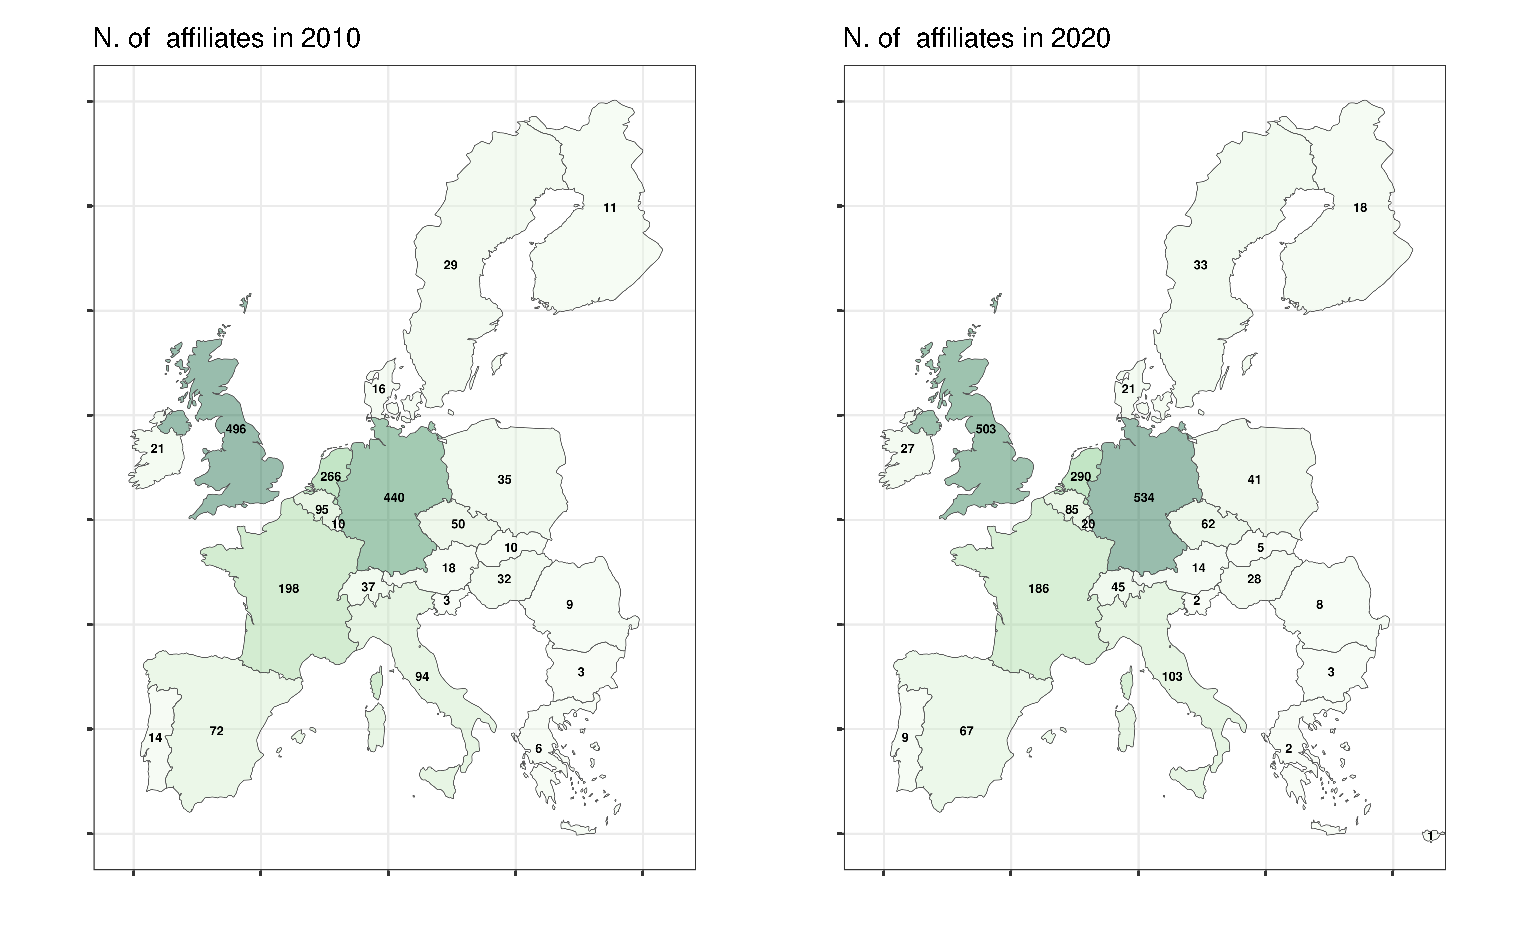
\includegraphics[keepaspectratio, scale=0.6]{FigA1-map-aff-2010-2020.eps}

  \caption{Location of Japanese affiliates in Europe}
    \label{fig:map}

\end{center}

\footnotesize
\emph{Source:} Authors' compilation based on Toyo Keizai's OJC data.\\
\emph{Note:} 
The figure shows the number of Japanese affiliates in European countries.

\end{figure}
% Des05_map.Rmd
% After making PDF plot, I converted it to EPS with online converter.
% https://convertio.co/pdf-eps/
%%%%%%%%%%%%%%%%%%%%%%%%%%%%%%%%%%%%%%%%%%%%%%%%%%%%%%%%



\clearpage
\section{Synthetic DiD Control Unit Weights}\label{sec:sdid_weights}

Table \ref{tab:sdid_weights} reports the synthetic DiD control unit weights aggregated by country, corresponding to the SDiD estimates shown in Figure \ref{fig:fig_SDiD-2} (affiliate exits) and Figure \ref{fig:fig_SDiD-entry} (new affiliate entries).


%%%%%%%%%%%%%%%%%%%%%%%%%%%%%%%%
{\renewcommand\normalsize{\scriptsize}%
\normalsize 
\begin{table}[!h]
\centering
\caption{\label{tab:sdid_weights}Synthetic DiD Control Unit Weights by Country}
\centering
\begin{tabular}[t]{lrr}
\toprule
Country & Exit & Entry\\
\midrule
Austria & 0.0150 & 0.0764\\
Belgium & 0.0792 & 0.0823\\
Denmark & 0.0135 & 0.0742\\
Finland & 0.0092 & 0.0789\\
France & 0.1652 & 0.1164\\
\addlinespace
Germany & 0.3669 & 0.1257\\
Ireland & 0.0177 & 0.0815\\
Italy & 0.0785 & 0.1008\\
Luxembourg & 0.0083 & 0.0830\\
Netherlands & 0.2220 & 0.1080\\
\addlinespace
Sweden & 0.0245 & 0.0728\\
\bottomrule
\end{tabular}
\end{table}

}
% Est11_Weight.Rmd
%%%%%%%%%%%%%%%%%%%%%%%%%%%%%%%%




\clearpage
\section{Asset Specificity}\label{sec:asset}

\cite{kermani2023asset} construct a novel dataset to measure asset specificity among nonfinancial firms, focusing on liquidation recovery rates (liquidation value relative to book value) across major industries. Using U.S. Chapter 11 bankruptcy filings from 2000 to 2018, they estimate that the average liquidation recovery rate for property, plant, and equipment (PPE) is 35\% (standard deviation 13\%).
They find that asset specificity, driven by physical attributes like mobility, customization, and durability, varies significantly across industries and impacts investment irreversibility, uncertainty effects.

\cite{kermani2023asset} provide a comprehensive dataset on liquidation recovery rates across industries. 
We assign the liquidation recovery rates from their Table II to the industries in the OJC dataset based on corresponding SIC codes. For OJC industries associated with multiple SIC codes, we calculate the average of the liquidation recovery rates of the relevant SIC codes. Following \cite{kermani2023asset}, who report an average PPE liquidation recovery rate of 0.35, we define industries with liquidation recovery rates above 0.35 as having low asset specificity, and those below 0.35 as having high asset specificity. This classification allows us to analyze the role of asset specificity within the OJC dataset.
Tables \ref{tab:SpecificityHigh} and \ref{tab:SpecificityLow} present the list of industries with high and low asset specificity, respectively.




%%%%%%%%%%%%%%%%%%%%%%%%%%%%%%%%
{\renewcommand\normalsize{\scriptsize}%
\normalsize 
\input{TableA4_AssetSpecificityH}
}
% LRR.do
% My Drive/my_working_papers/2024Brexit/
%%%%%%%%%%%%%%%%%%%%%%%%%%%%%%%%


%%%%%%%%%%%%%%%%%%%%%%%%%%%%%%%%
{\renewcommand\normalsize{\scriptsize}%
\normalsize 
\input{TableA5_AssetSpecificityL}
}
% LRR.do
% My Drive/my_working_papers/2024Brexit/
%%%%%%%%%%%%%%%%%%%%%%%%%%%%%%%%



\end{document}


